\documentclass{article}
\usepackage{graphicx}
\usepackage{sectsty}
\usepackage{dirtree}
\usepackage[export]{adjustbox}
\usepackage{hyperref}

\hypersetup{
    colorlinks=true,
    linkcolor=blue,
    urlcolor=blue,
}

\sectionfont{\centering}

\title{Angry-Birds-using-Pygame}
\author{Tamanna Kumari}
\date{A CS104 Project Spring 2024-25}

\begin{document}
\maketitle
\tableofcontents
\newpage

\section{INTRODUCTION}
This is a two-player Angry Birds Showdown. First one to destroy all of the opponent's blocks wins. All the birds have their own unique special ability and induce variable damage based on their type, speed etc.

\section{About the birds}
\begin{center}
    \textbf{RIGHT MOUSE CLICK ACTIVATES SPECIAL ABILITIES.}
\end{center}


\begin{figure}[h!]
    \centering
    
\includegraphics[width = 0.2\textwidth]{../Resources/red.png}
    \caption{RED}
    \label{fig : RED}
\end{figure}

\subsection{RED}

Red does equal damage to all the blocks for a given speed.

Special Ability : It can transform into giant red which is very very powerful and does maximum damage possible. 

Usage : It's special ability can be only used once per player.


\begin{figure}[h!]
    \centering
    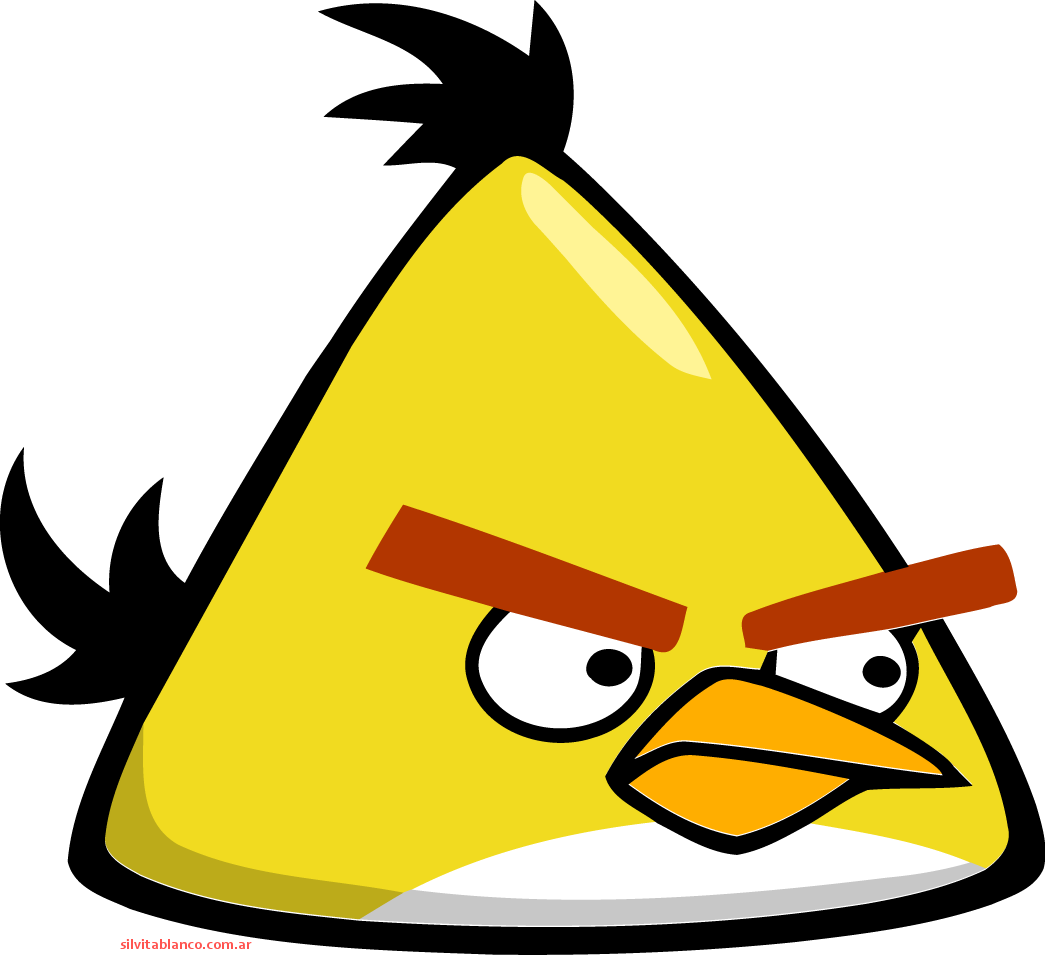
\includegraphics[width = 0.2\textwidth]{../Resources/fast_yellow.png}
    \caption{CHUCK}
    \label{fig : CHUCK}
\end{figure}
\subsection{CHUCK}


Chuck does more damage to wood blocks and less damage to others for a given speed.

Special Ability : Super Speed
It attains really high speed which increases it's damage.

Usage : Unlimited. A player can use it's special ability everytime.

\subsection{BLUE}
\begin{figure}[h!]
    \centering
    
\includegraphics[width = 0.2\textwidth]{../Resources/small_blue.png}
    \caption{BLUE}
    \label{fig : BLUE}
\end{figure}


Blue does more damage to ice blocks and less damage to others for the same speed.

Special Ability : Triplify
It can multiply into 3 and triple it's attack area and increase damage.

Usage : Unlimited. A player can use it's special ability everytime.




\begin{figure}[h!]
    \centering
    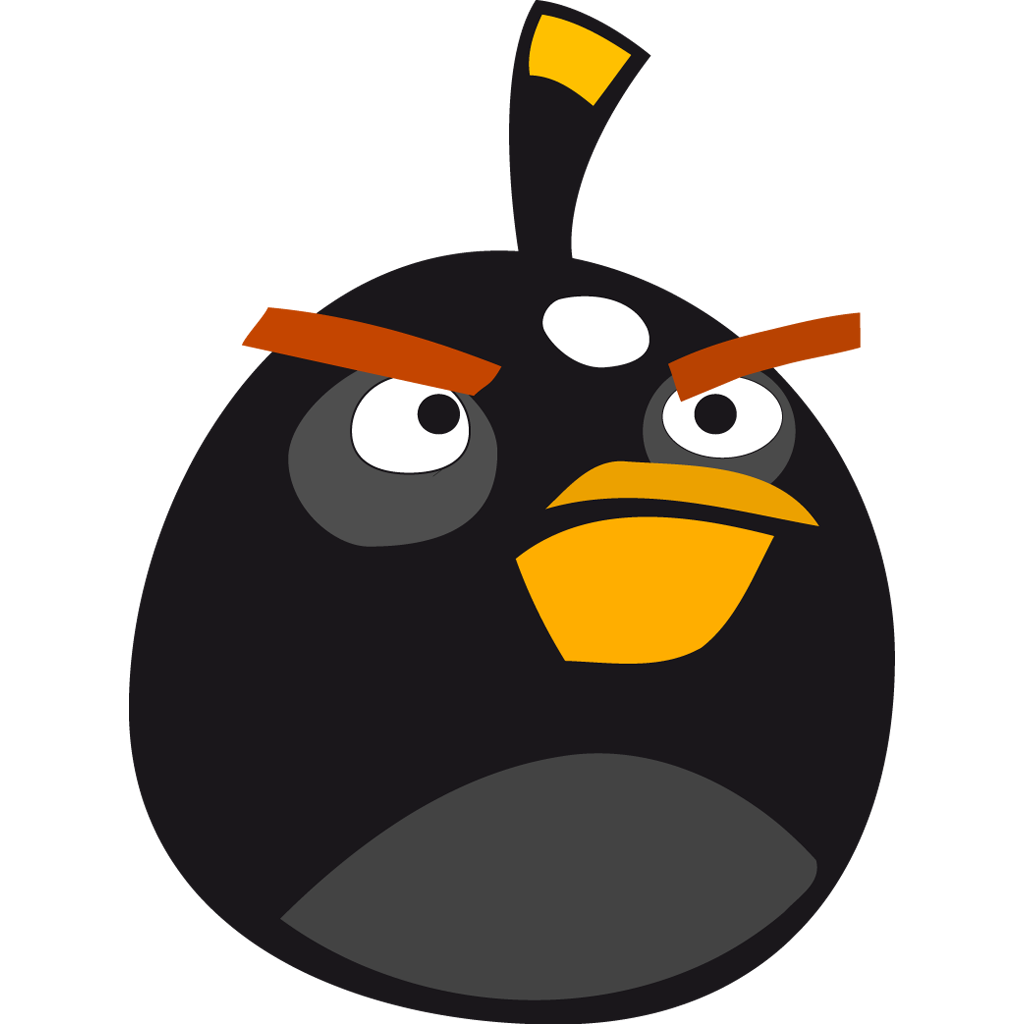
\includegraphics[width = 0.2\textwidth]{../Resources/bomb.png}
    \caption{BOMB}
    \label{fig : BOMB}
\end{figure}
\subsection{BOMB}
Bomb does more damage to stone blocks and less damage to others for the same speed.

Special Ability : Bomb
It can burst upon collision and induce heavy damage on all the blocks. 

Usage : It's usage is a gamble. Both players combined can use this ability a total of n times where n is a randomly generated number in the range of 0 to 5. So it may happen that neither player gets to use this ability in a match. Moreover you must time your usage of this ability as the number of times you can use it also depends upon your opponent.

\section{MODULES}
\begin{description}
    \item[pygame-ce]: An actively maintained and updated version of the original pygame library offering enhanced support, bug-fixes and compatability with modern python versions for game-dev. This module has been used throughout the game 
    \item[random]: The random module in Python implements pseudo-random number generators for various distributions, and also provides functions for random operations on sequences, such as shuffling. I have used this module at instances such as random player activation and assigning maximum bomb ability usage.
    \item[os]: The os module in Python provides functions for interacting with the operating system. I have used it for the new-game button that restarts the program.
    \item[sys]: The sys module in Python provides access to system-specific parameters and functions, enabling interaction with the Python runtime environment. This again I used for new-game button and to terminate the current program.
    \item[math]: The math module in Python is a built-in library providing access to a wide range of mathematical functions and constants. I have used it to get access to trigonometric functions and add modifications to the projectile. 
\end{description}

\section{DIRECTORY STRUCTURE}

\dirtree{%
.1 \hspace{1.5pt}..
.2 Modules.
.3 birds.py.
.3 blocks.py.
.3 Buttons.py.
.3 players.py.
.2 Resources.
.3 audio.
.3 Fonts.
.2 main.py.
.2 initialized.py.
.2 working.py.
.2 requirements.txt.
}

\begin{itemize}
    \item \textbf{Modules}: It contains programs that control major part of the game.
    \item \textbf{Resources}: All the audio, images, fonts used in the game.
    \item \textbf{main.py} : The main Game loop.
    \item \textbf{initialized.py}: All the initialization of variables and class instances are here.
    \item \textbf{working.py}: It contains all the functions needed for the working of the game.
\end{itemize}

\section{Running Instruction}
\subsection{Pre-Requisites}
\textbf{Assuming python is already installed}

Run the following commands in order to create a virtual environment to run the game

\texttt{python -m venv venv} or \texttt{python3 -m venv venv}

\texttt{source venv/bin/activate}

\texttt{python -m pip install -r requirements.txt}

Game can be run by using

\texttt{python3 main.py > /dev/null}

or

\texttt{python main.py > /dev/null}

\subsection{Game Navigation and GamePlay}
\subsubsection{Loading Screen}
\begin{figure}[h!]
    \centering
    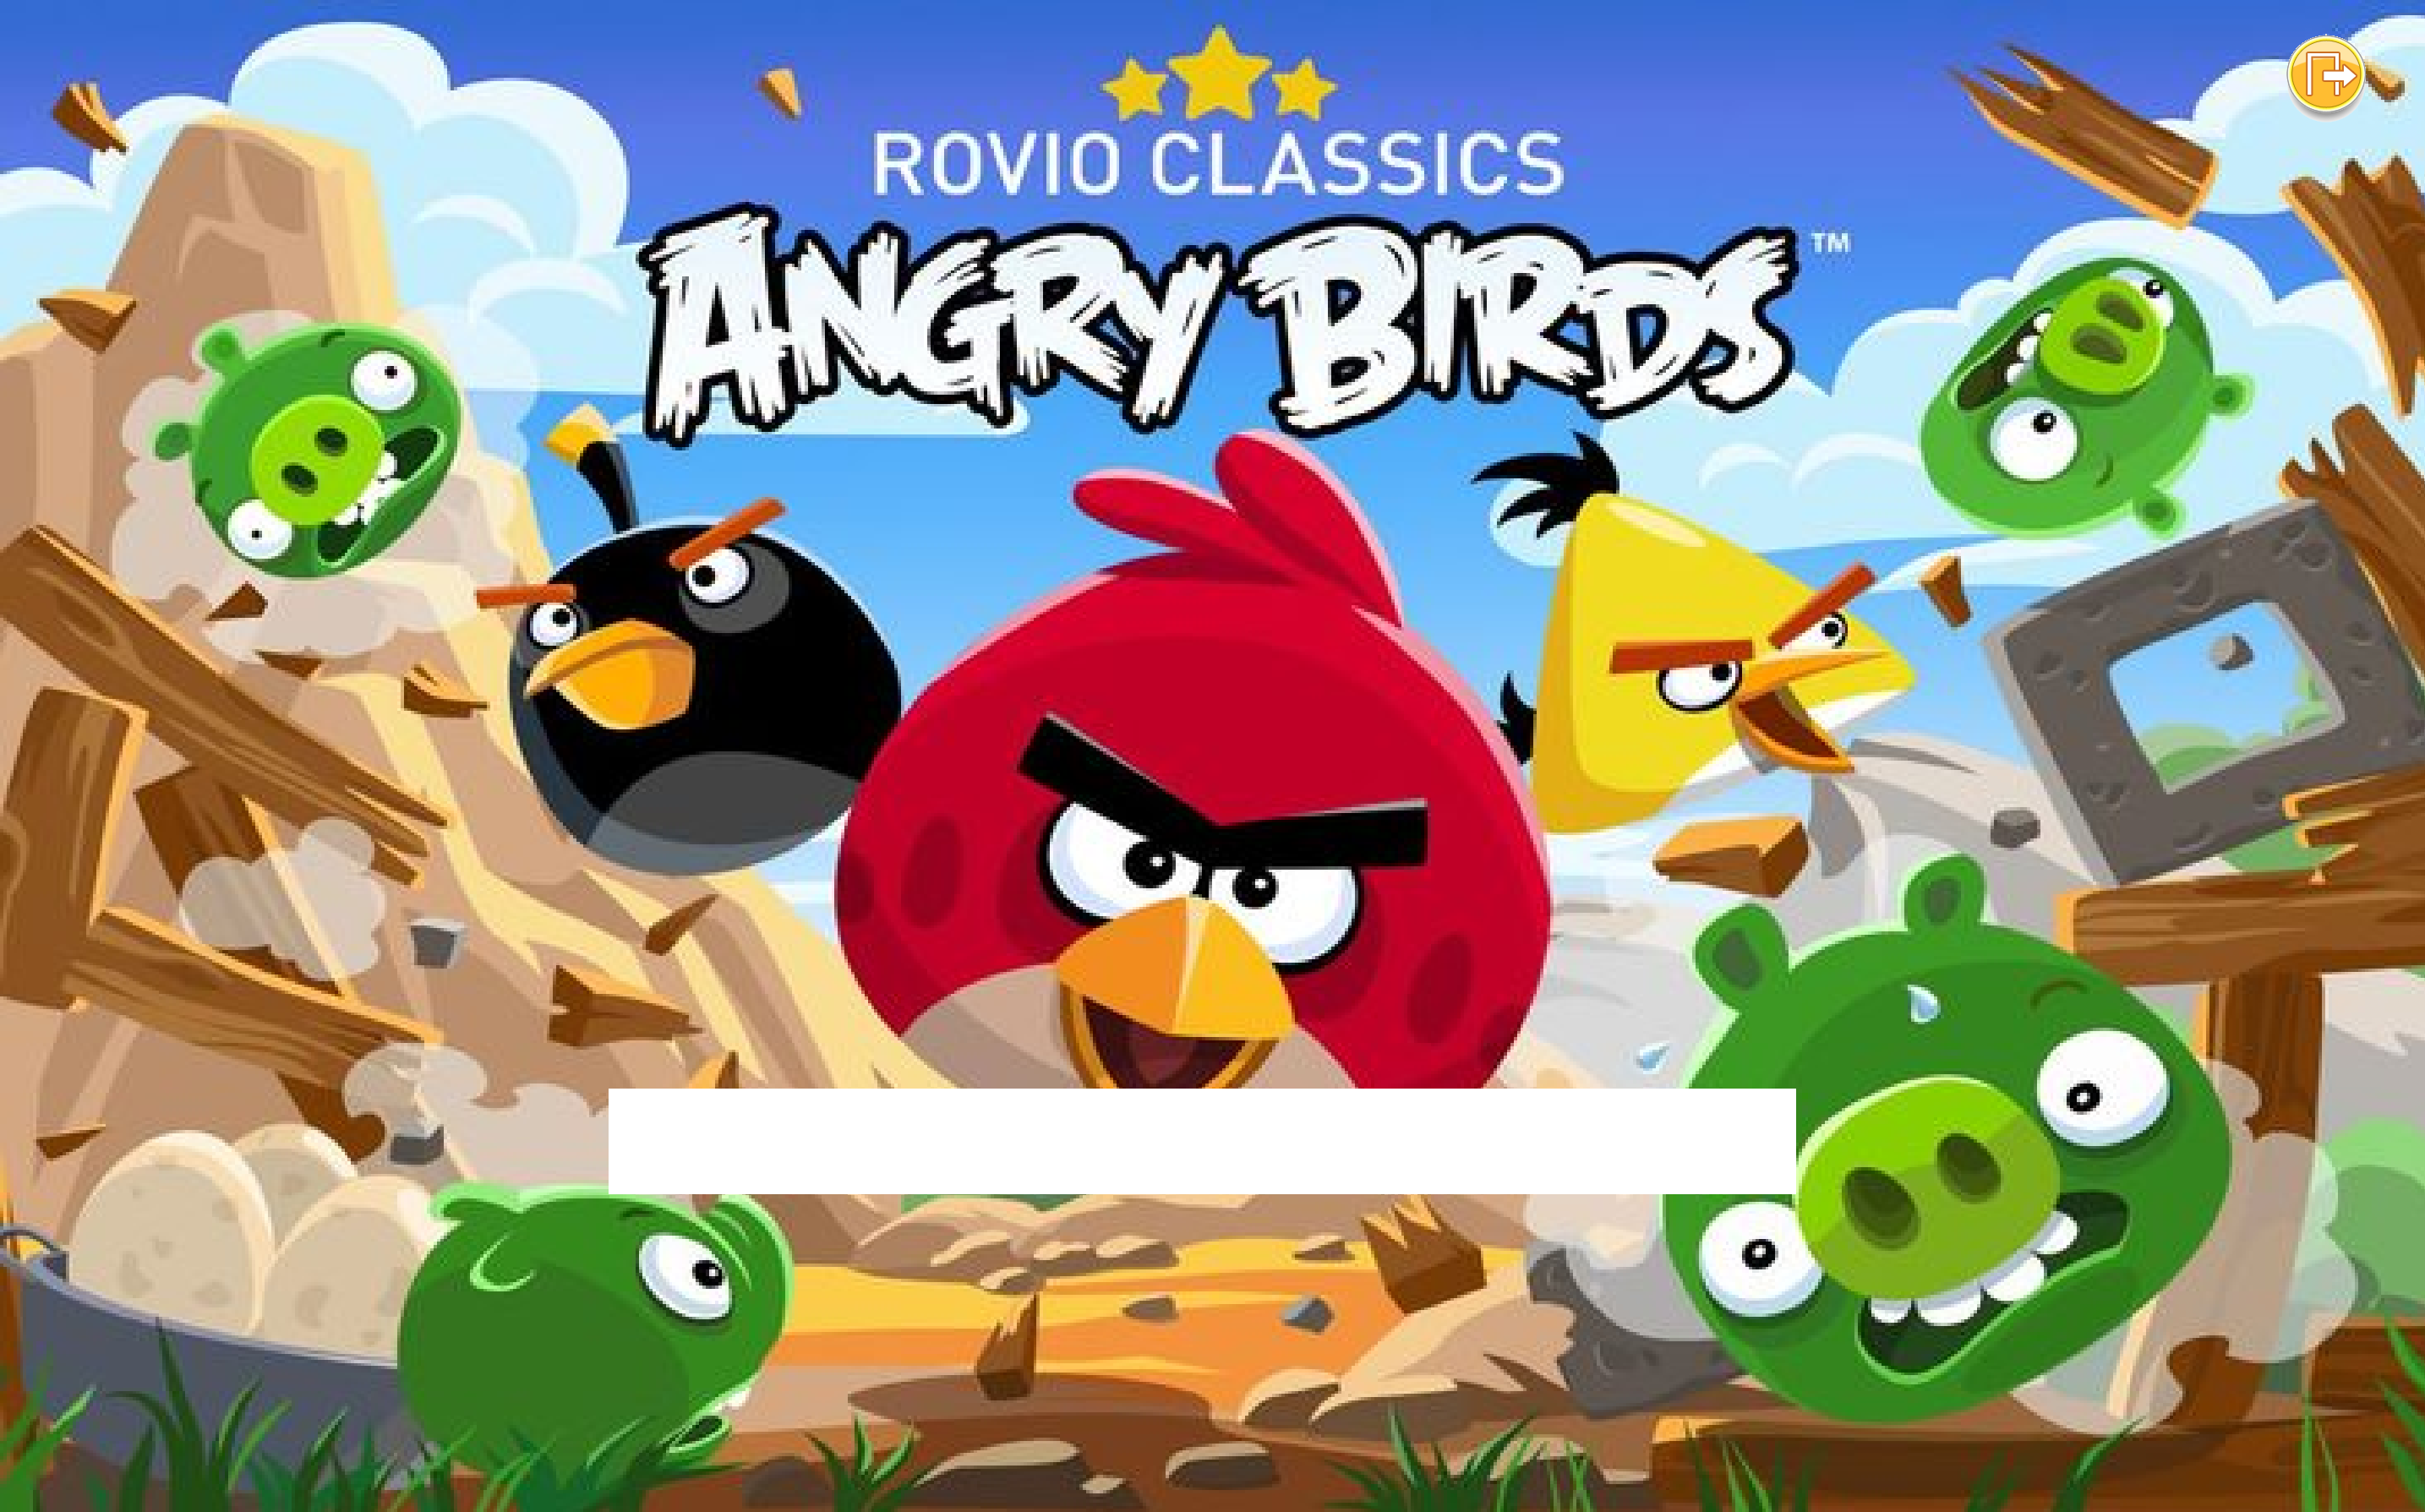
\includegraphics[width = 1.0\textwidth]{loading_screen.png}
    \caption{LOADING SCREEN}
    \label{fig:LOADING SCREEN}
\end{figure}

\subsubsection{Game Start}


\begin{itemize}
    \item \textbf{PLAY BUTTON}: Click to begin the game.
    \item \textbf{QUIT BUTTON}: On the upper right corner. Click to exit the game.
\end{itemize}

\begin{figure}[h!]
    \centering
    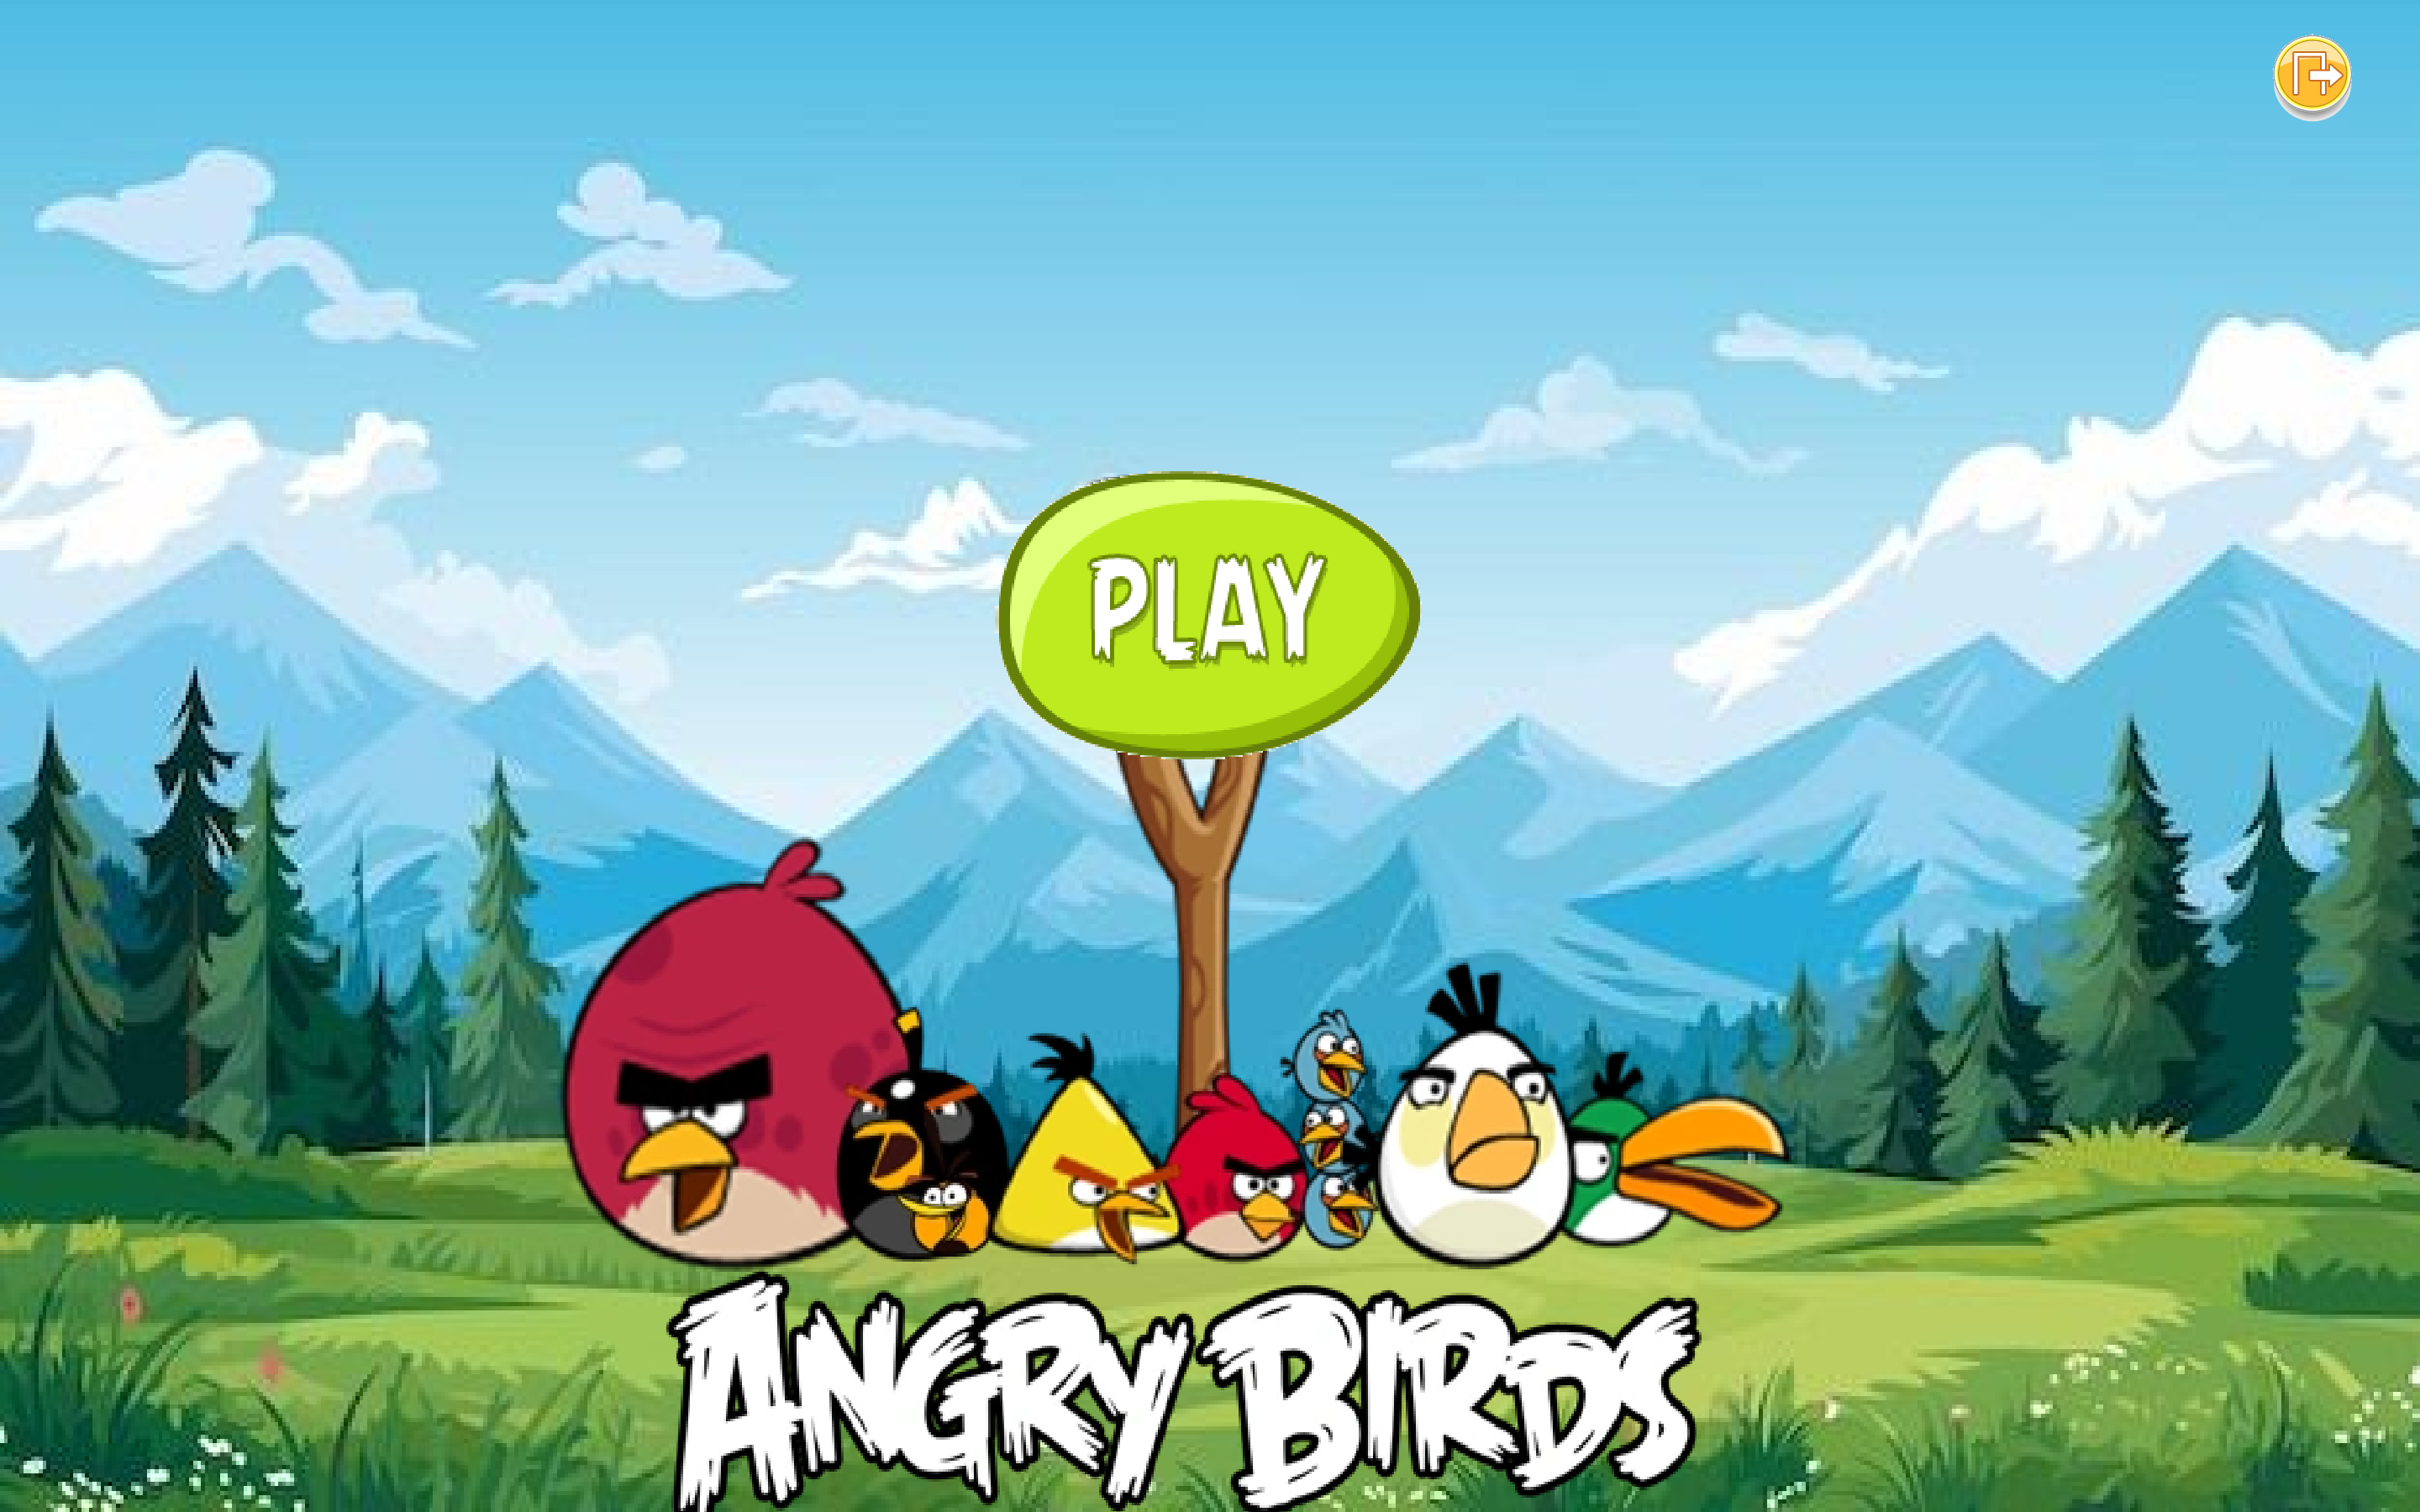
\includegraphics[width = 1.0\textwidth]{play_button.png}
    \caption{MAIN MENU}
    \label{fig:MAIN_MENU}
\end{figure}


\subsubsection{Player Name Input} 
Click on the desired input box to type the player name. 
Press "ENTER" and the name will pop up on the player's side of the screen

\begin{figure}[h]
    \begin{minipage}[b]{0.45\linewidth}
        \centering
        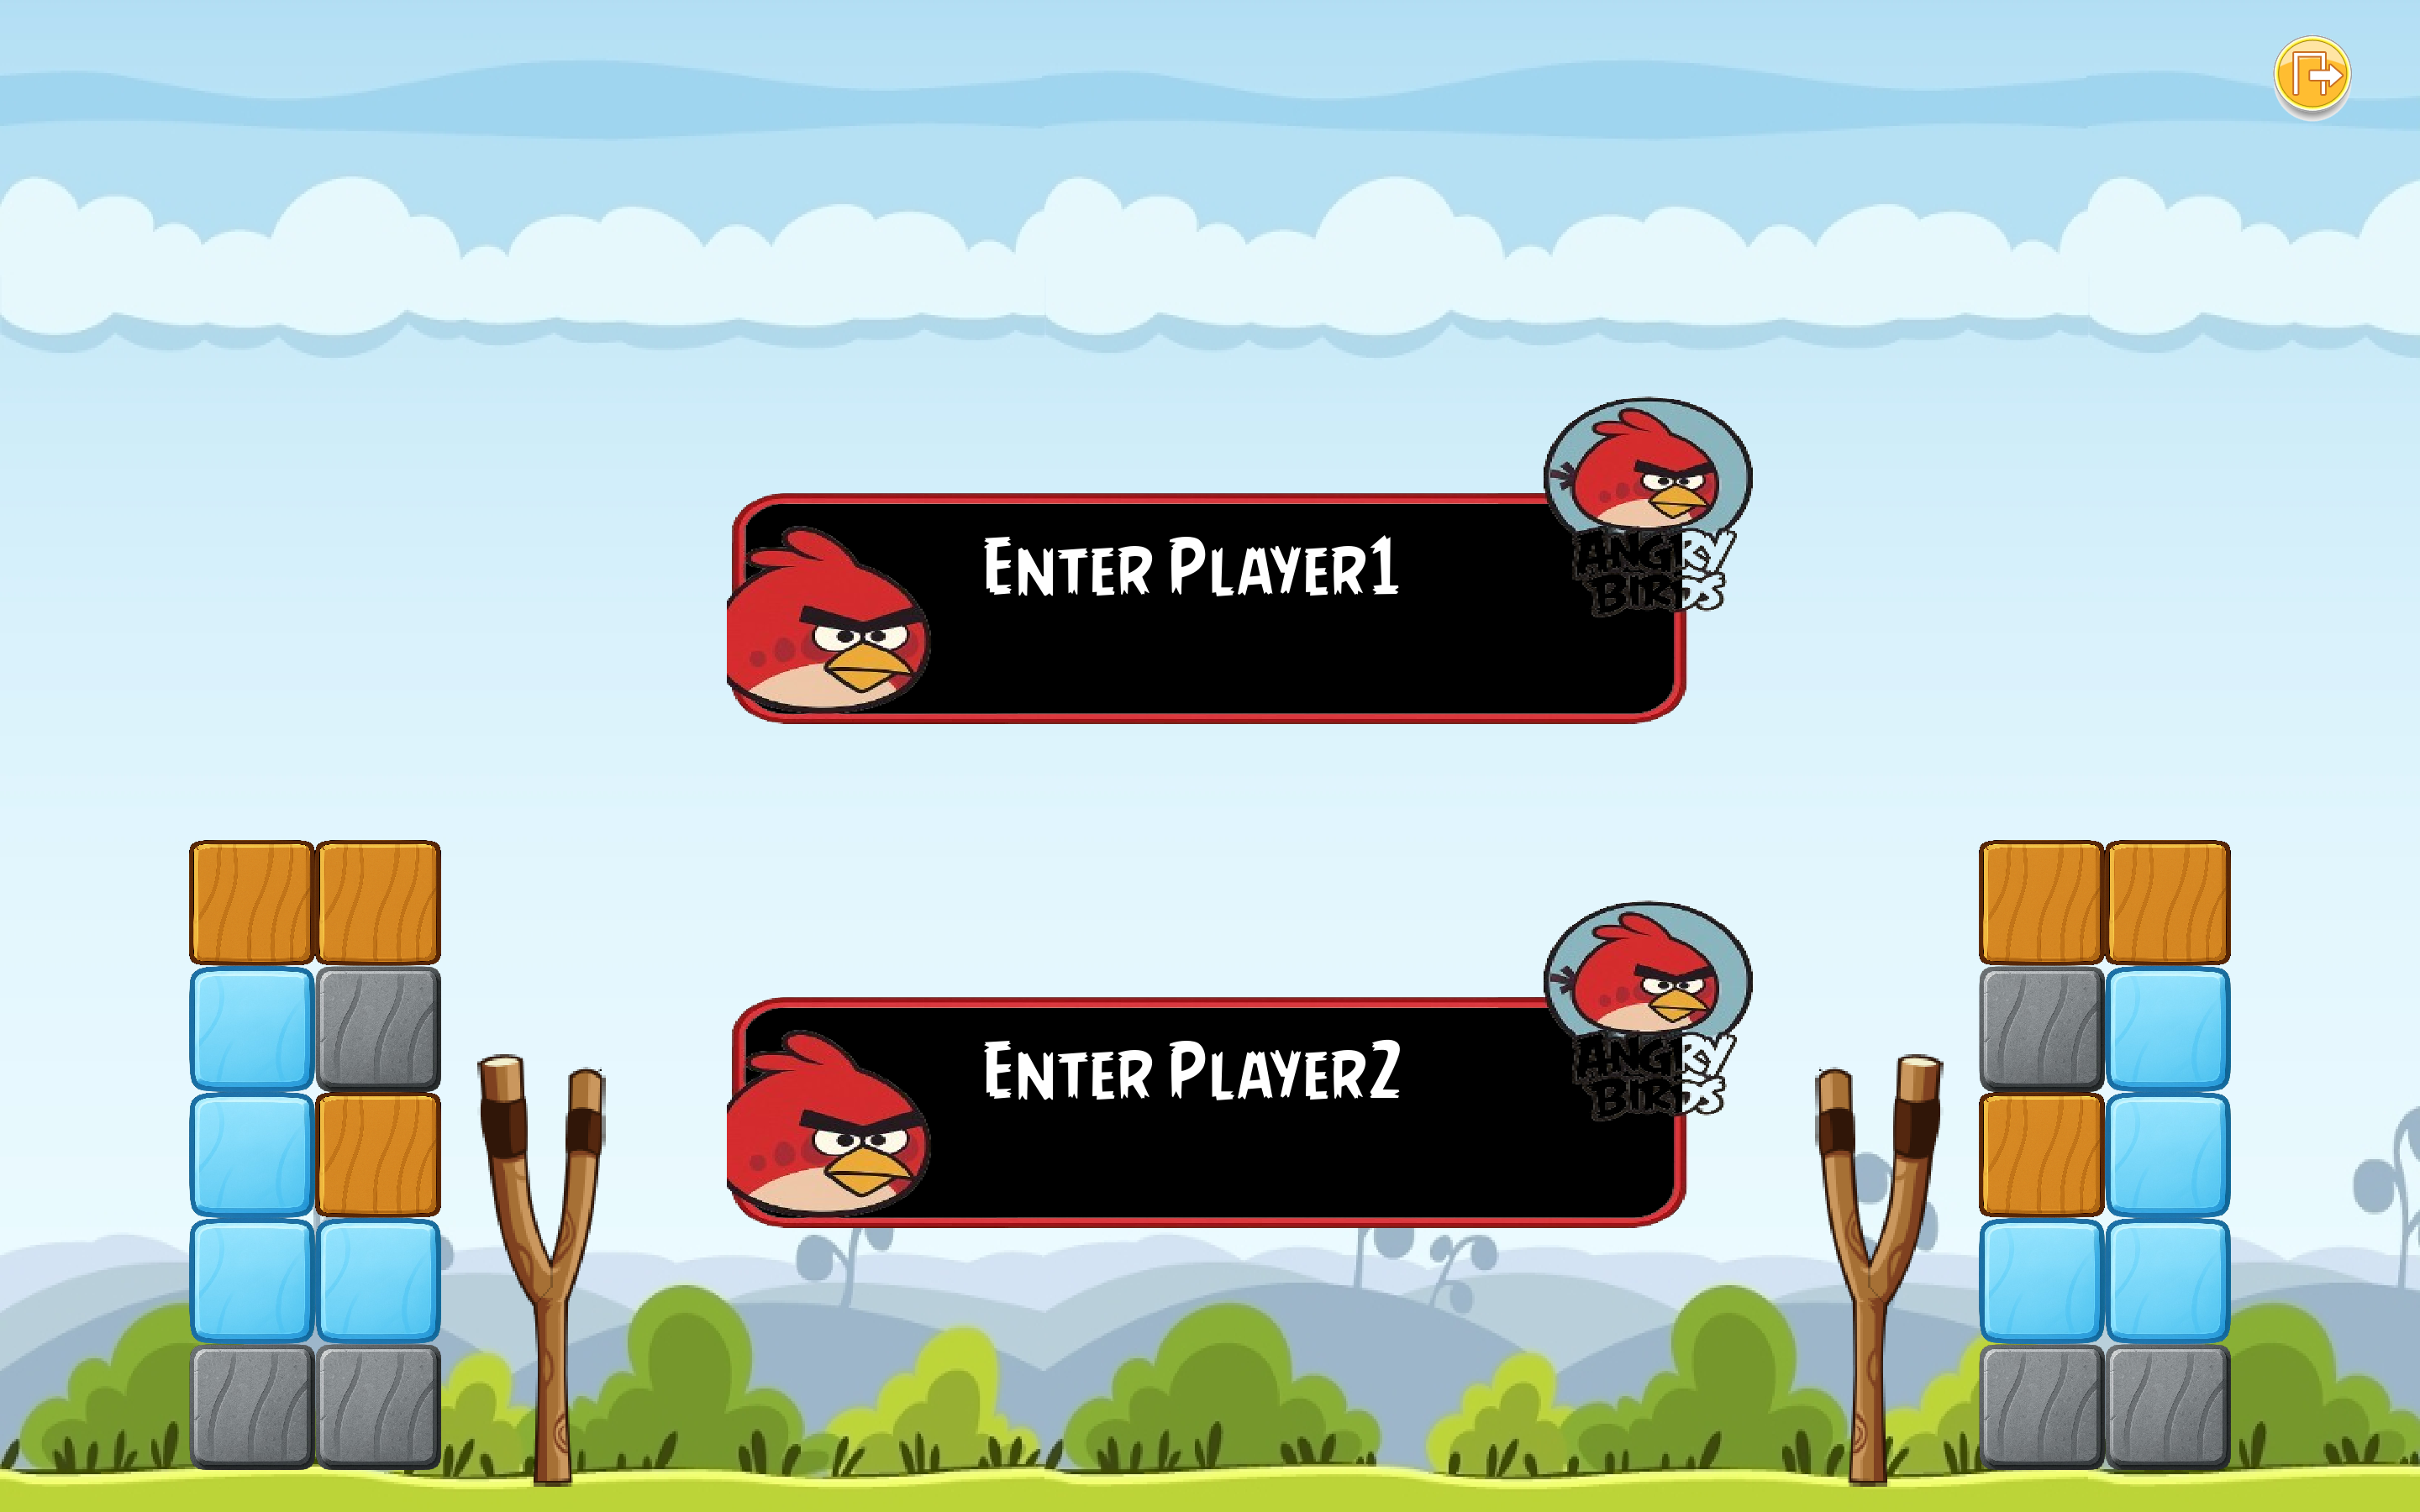
\includegraphics[width = 1\textwidth,left]{enter_players.png}
    \end{minipage}
    \hspace{0.25\textwidth}
    \begin{minipage}[b]{0.45\linewidth}
        \centering
        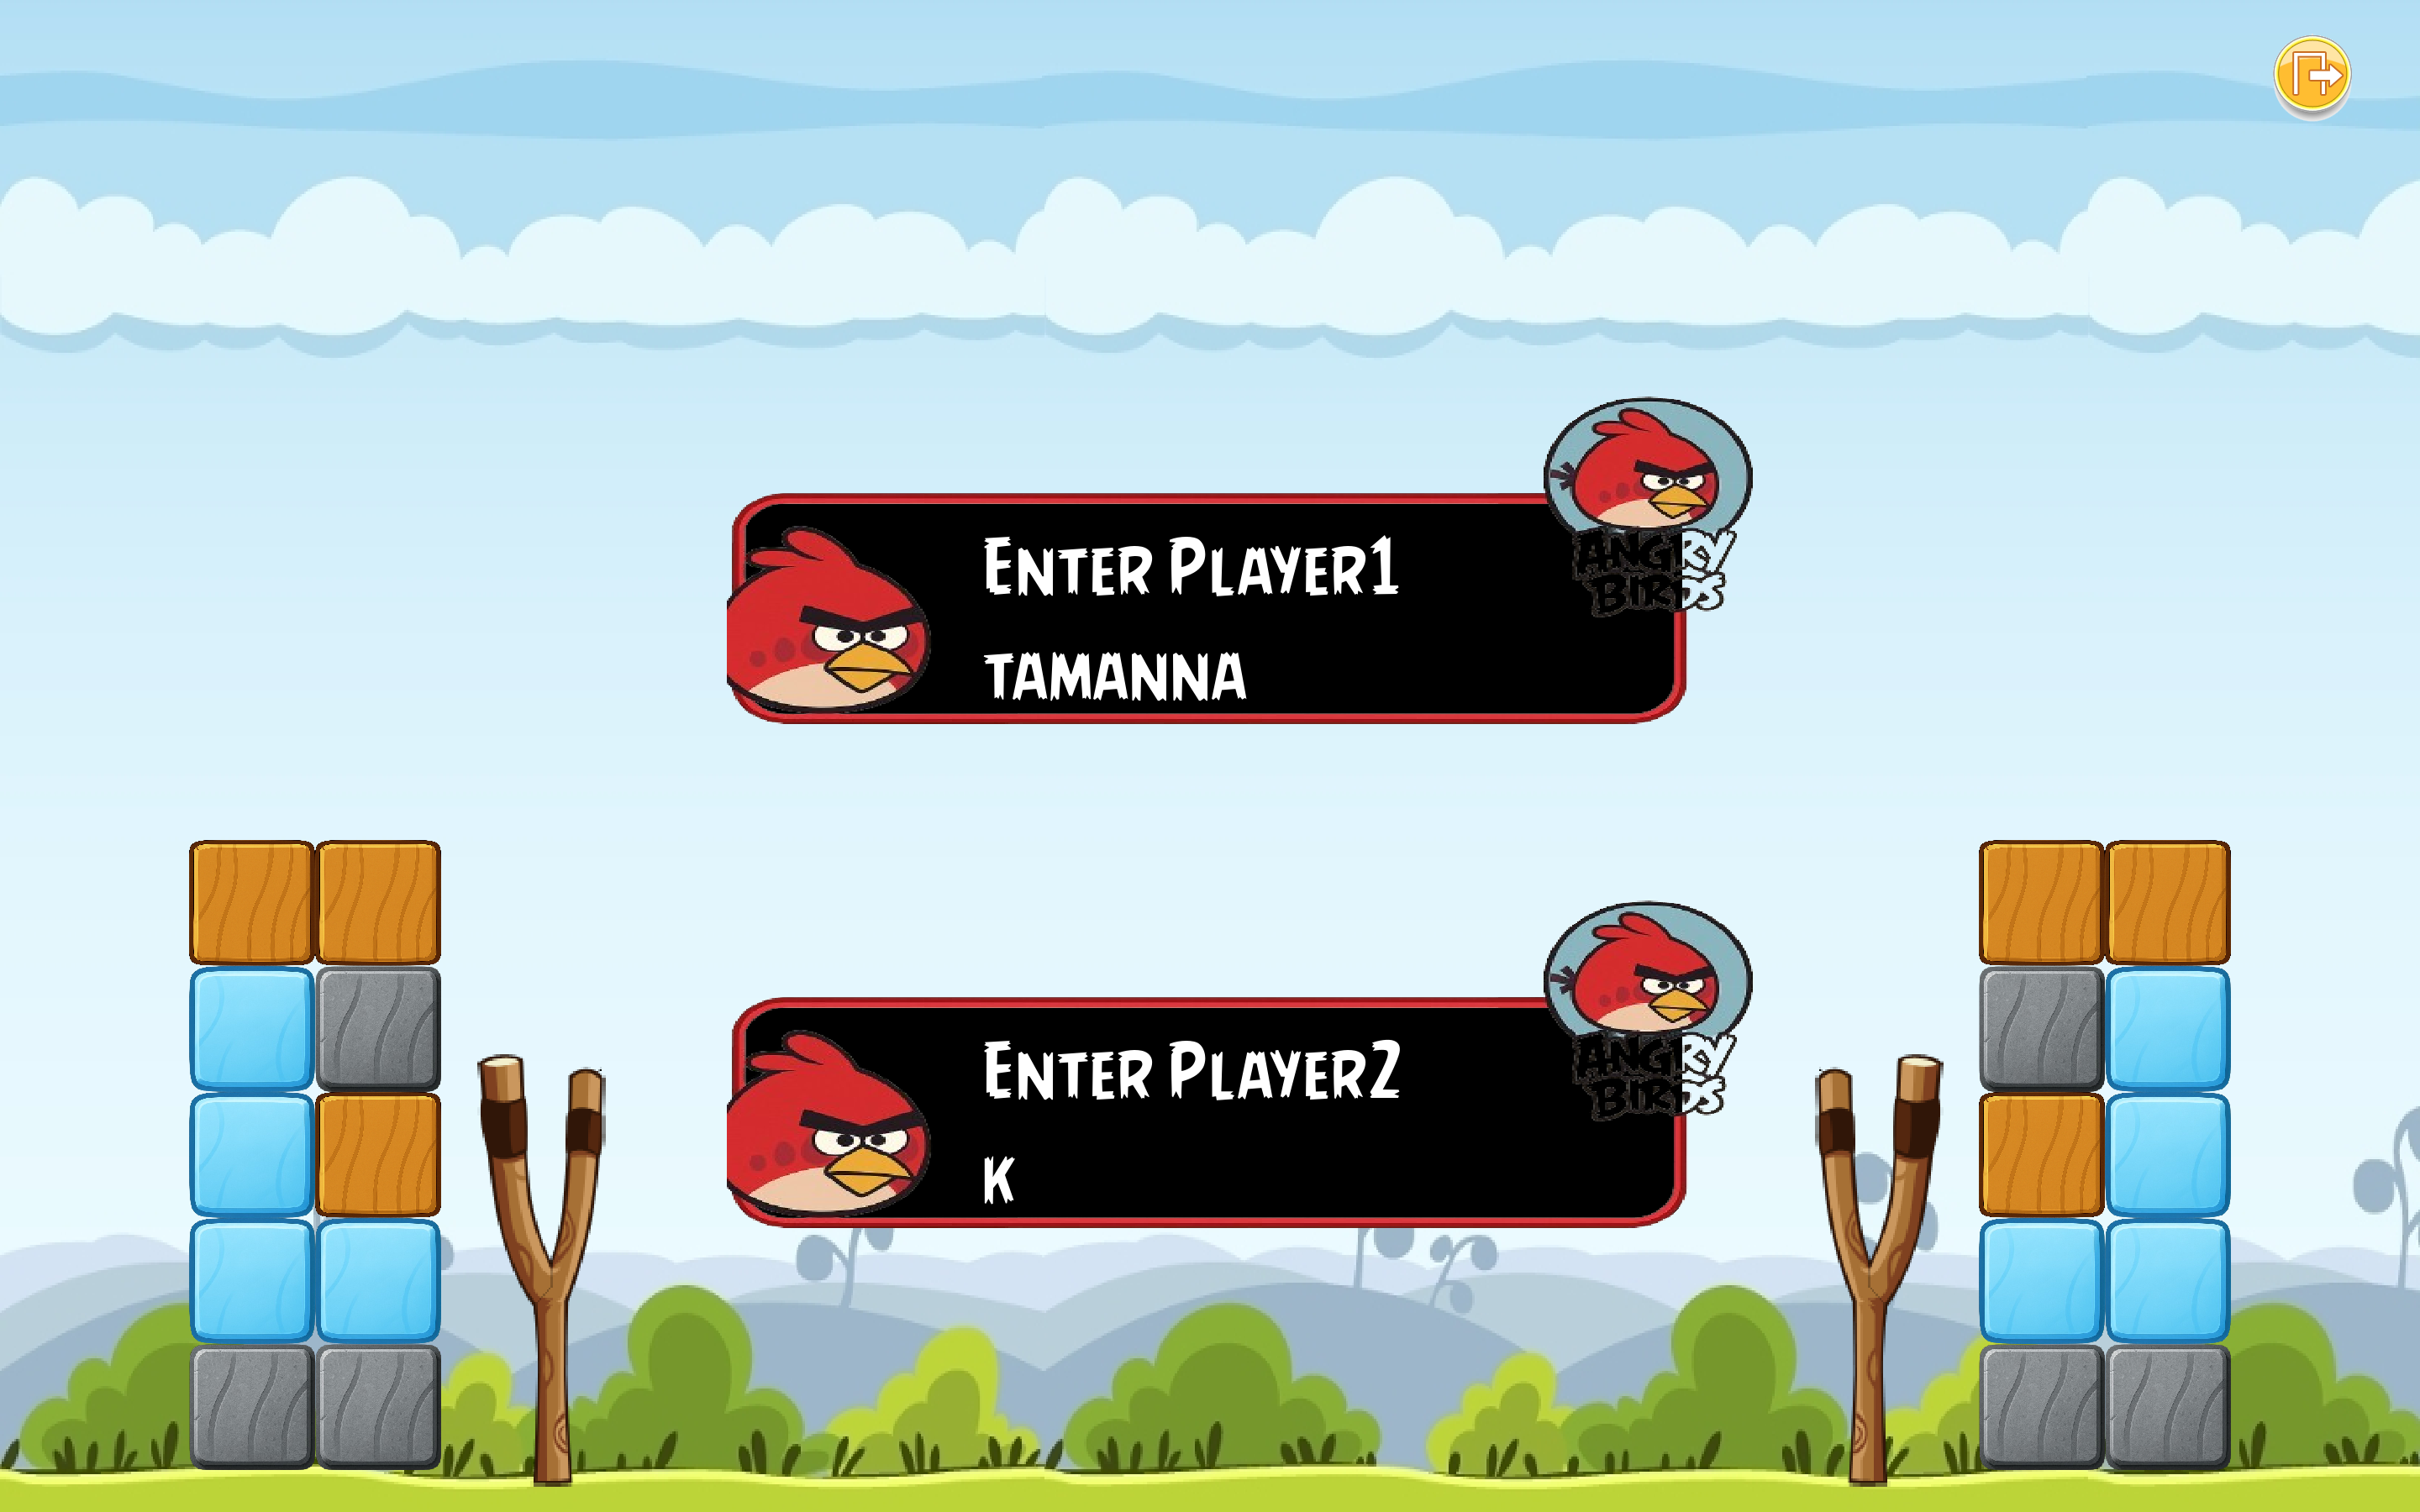
\includegraphics[width = 1\textwidth,left]{entering_players.png}
    \end{minipage}
    \caption{PLAYER NAME INPUT}
    \label{fig:PLAYER_NAME_INPUT}
\end{figure}

\newpage
\subsubsection{Choose Birds}

Each player clicks on their desired bird. Per player a maximum of 3 birds are allowed.
Hovering over a bird opens the bird description.
\begin{figure}[h!]
    \centering
    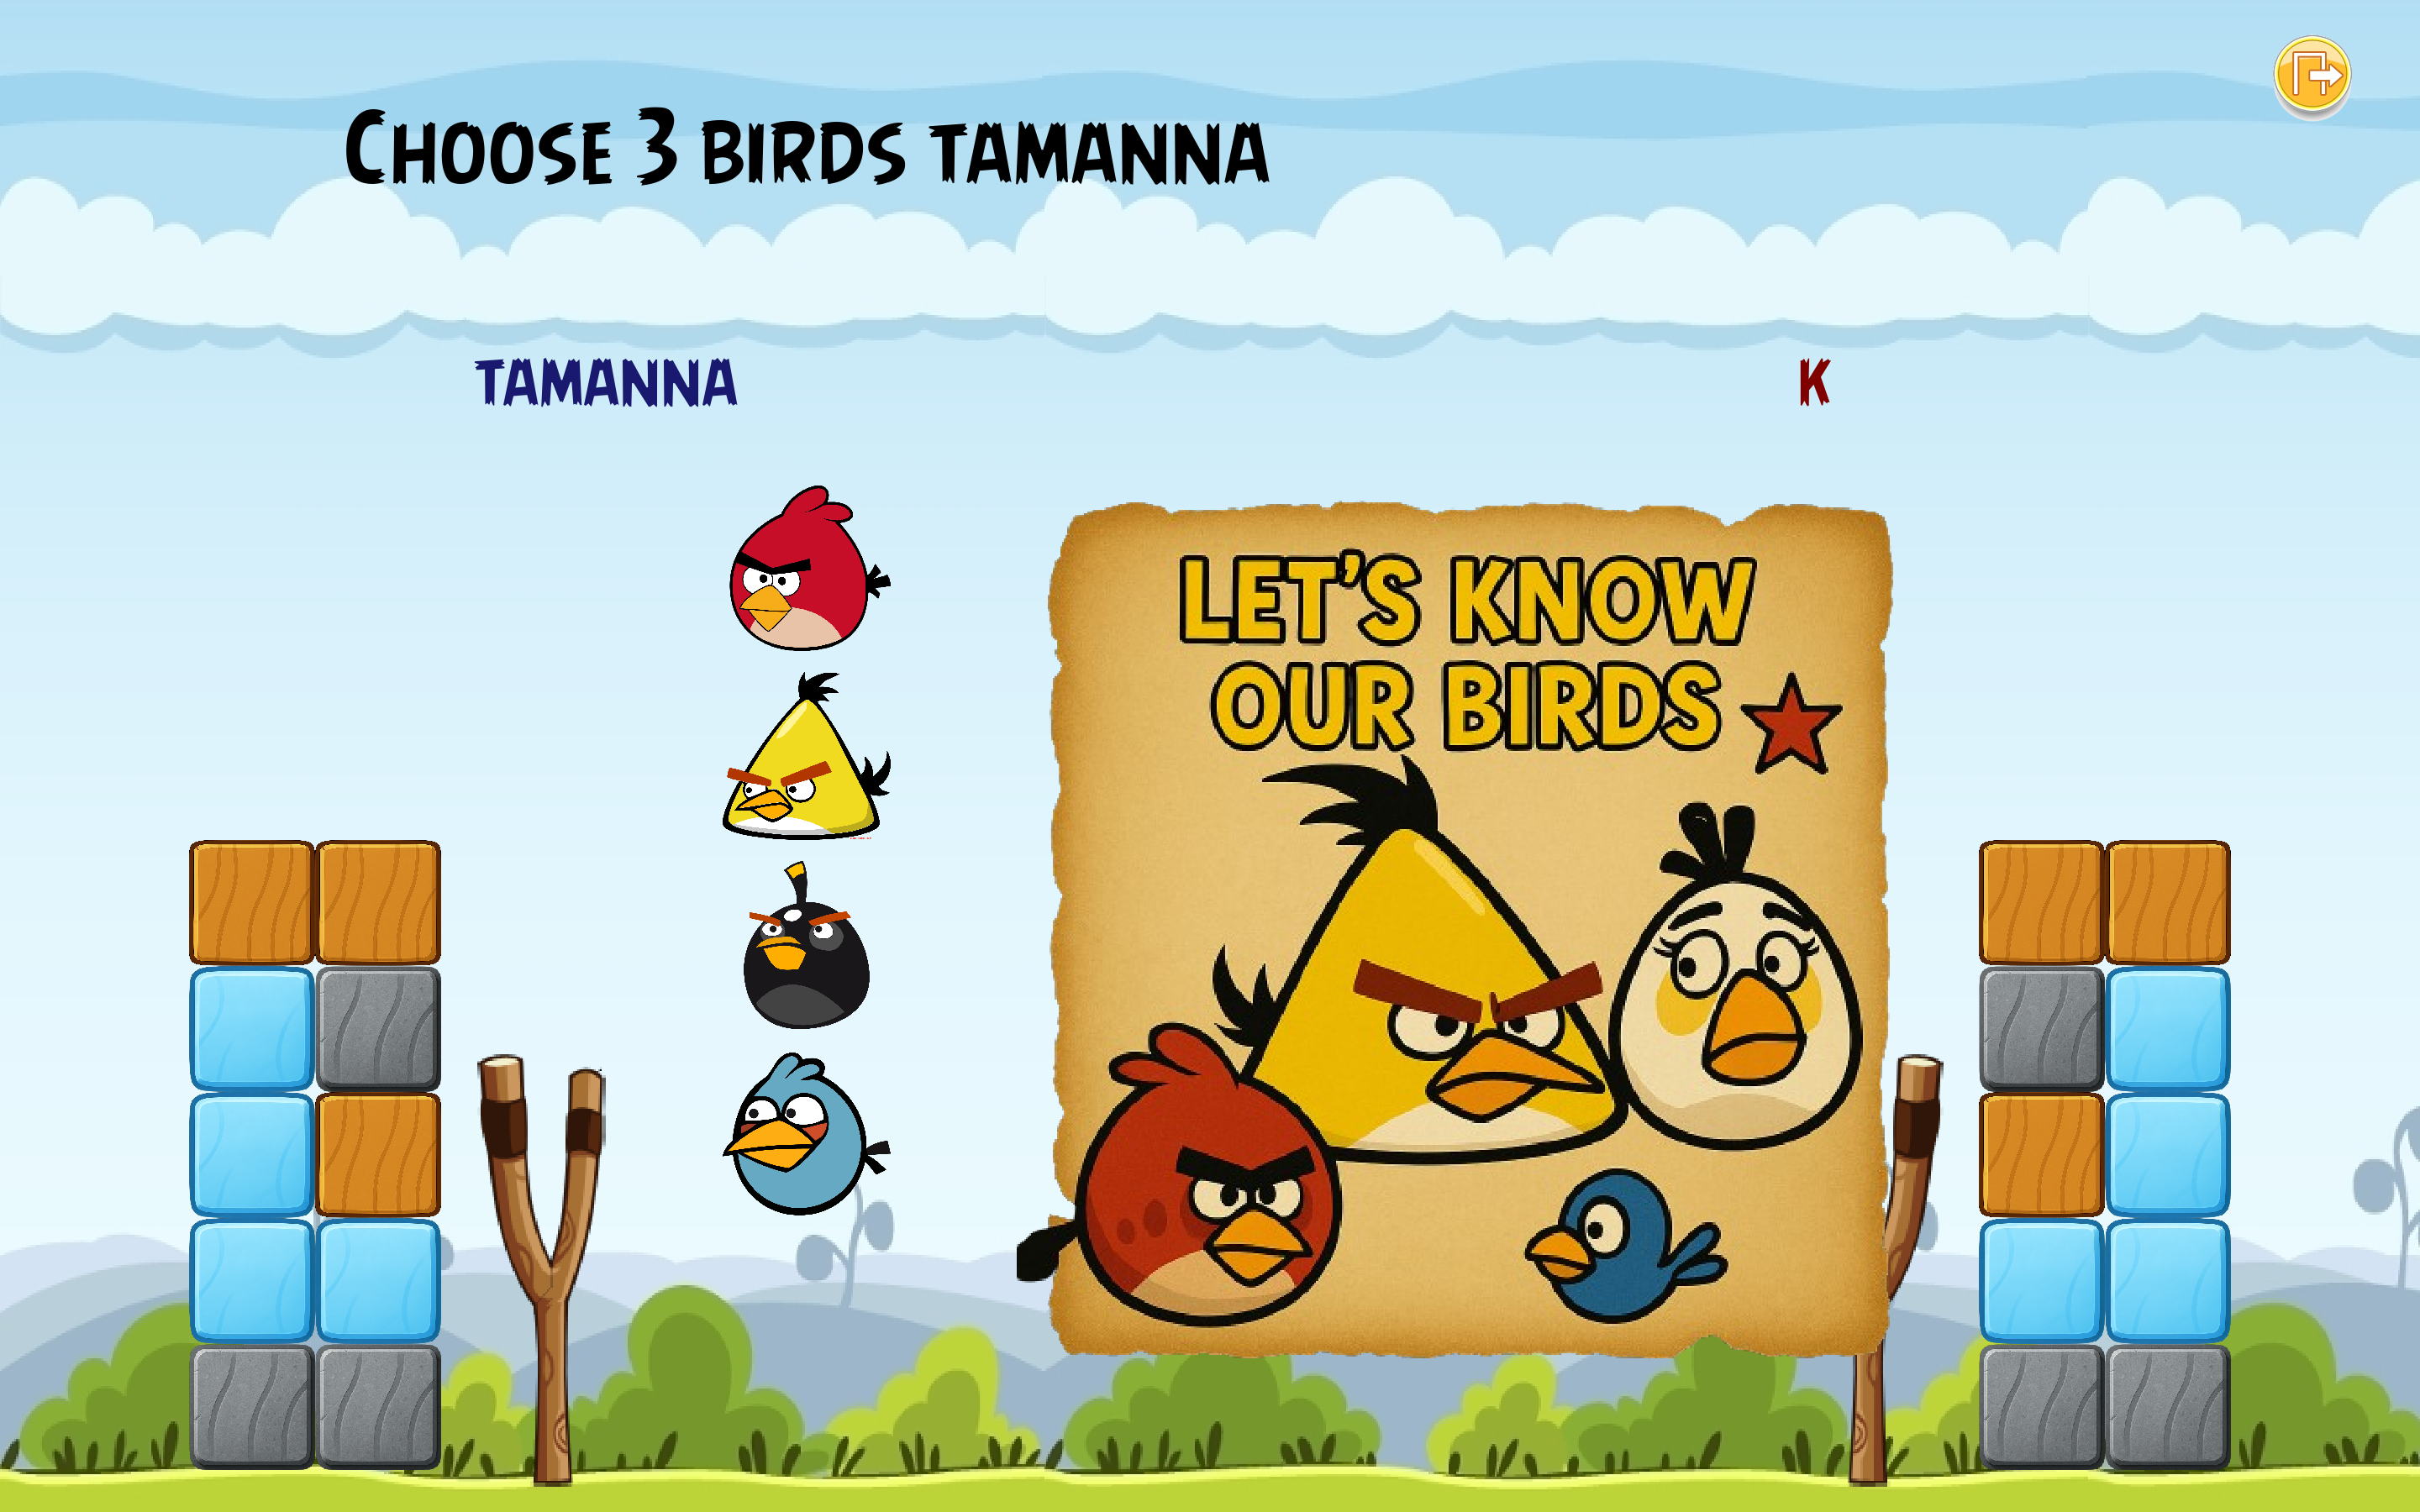
\includegraphics[width = 1.0\textwidth]{choose_birds.png}
    \caption{BIRD MENU}
    \label{fig:BIRD_MENU}
\end{figure}

\subsection{Player VS Player}

\begin{figure}[h!]
    \centering
    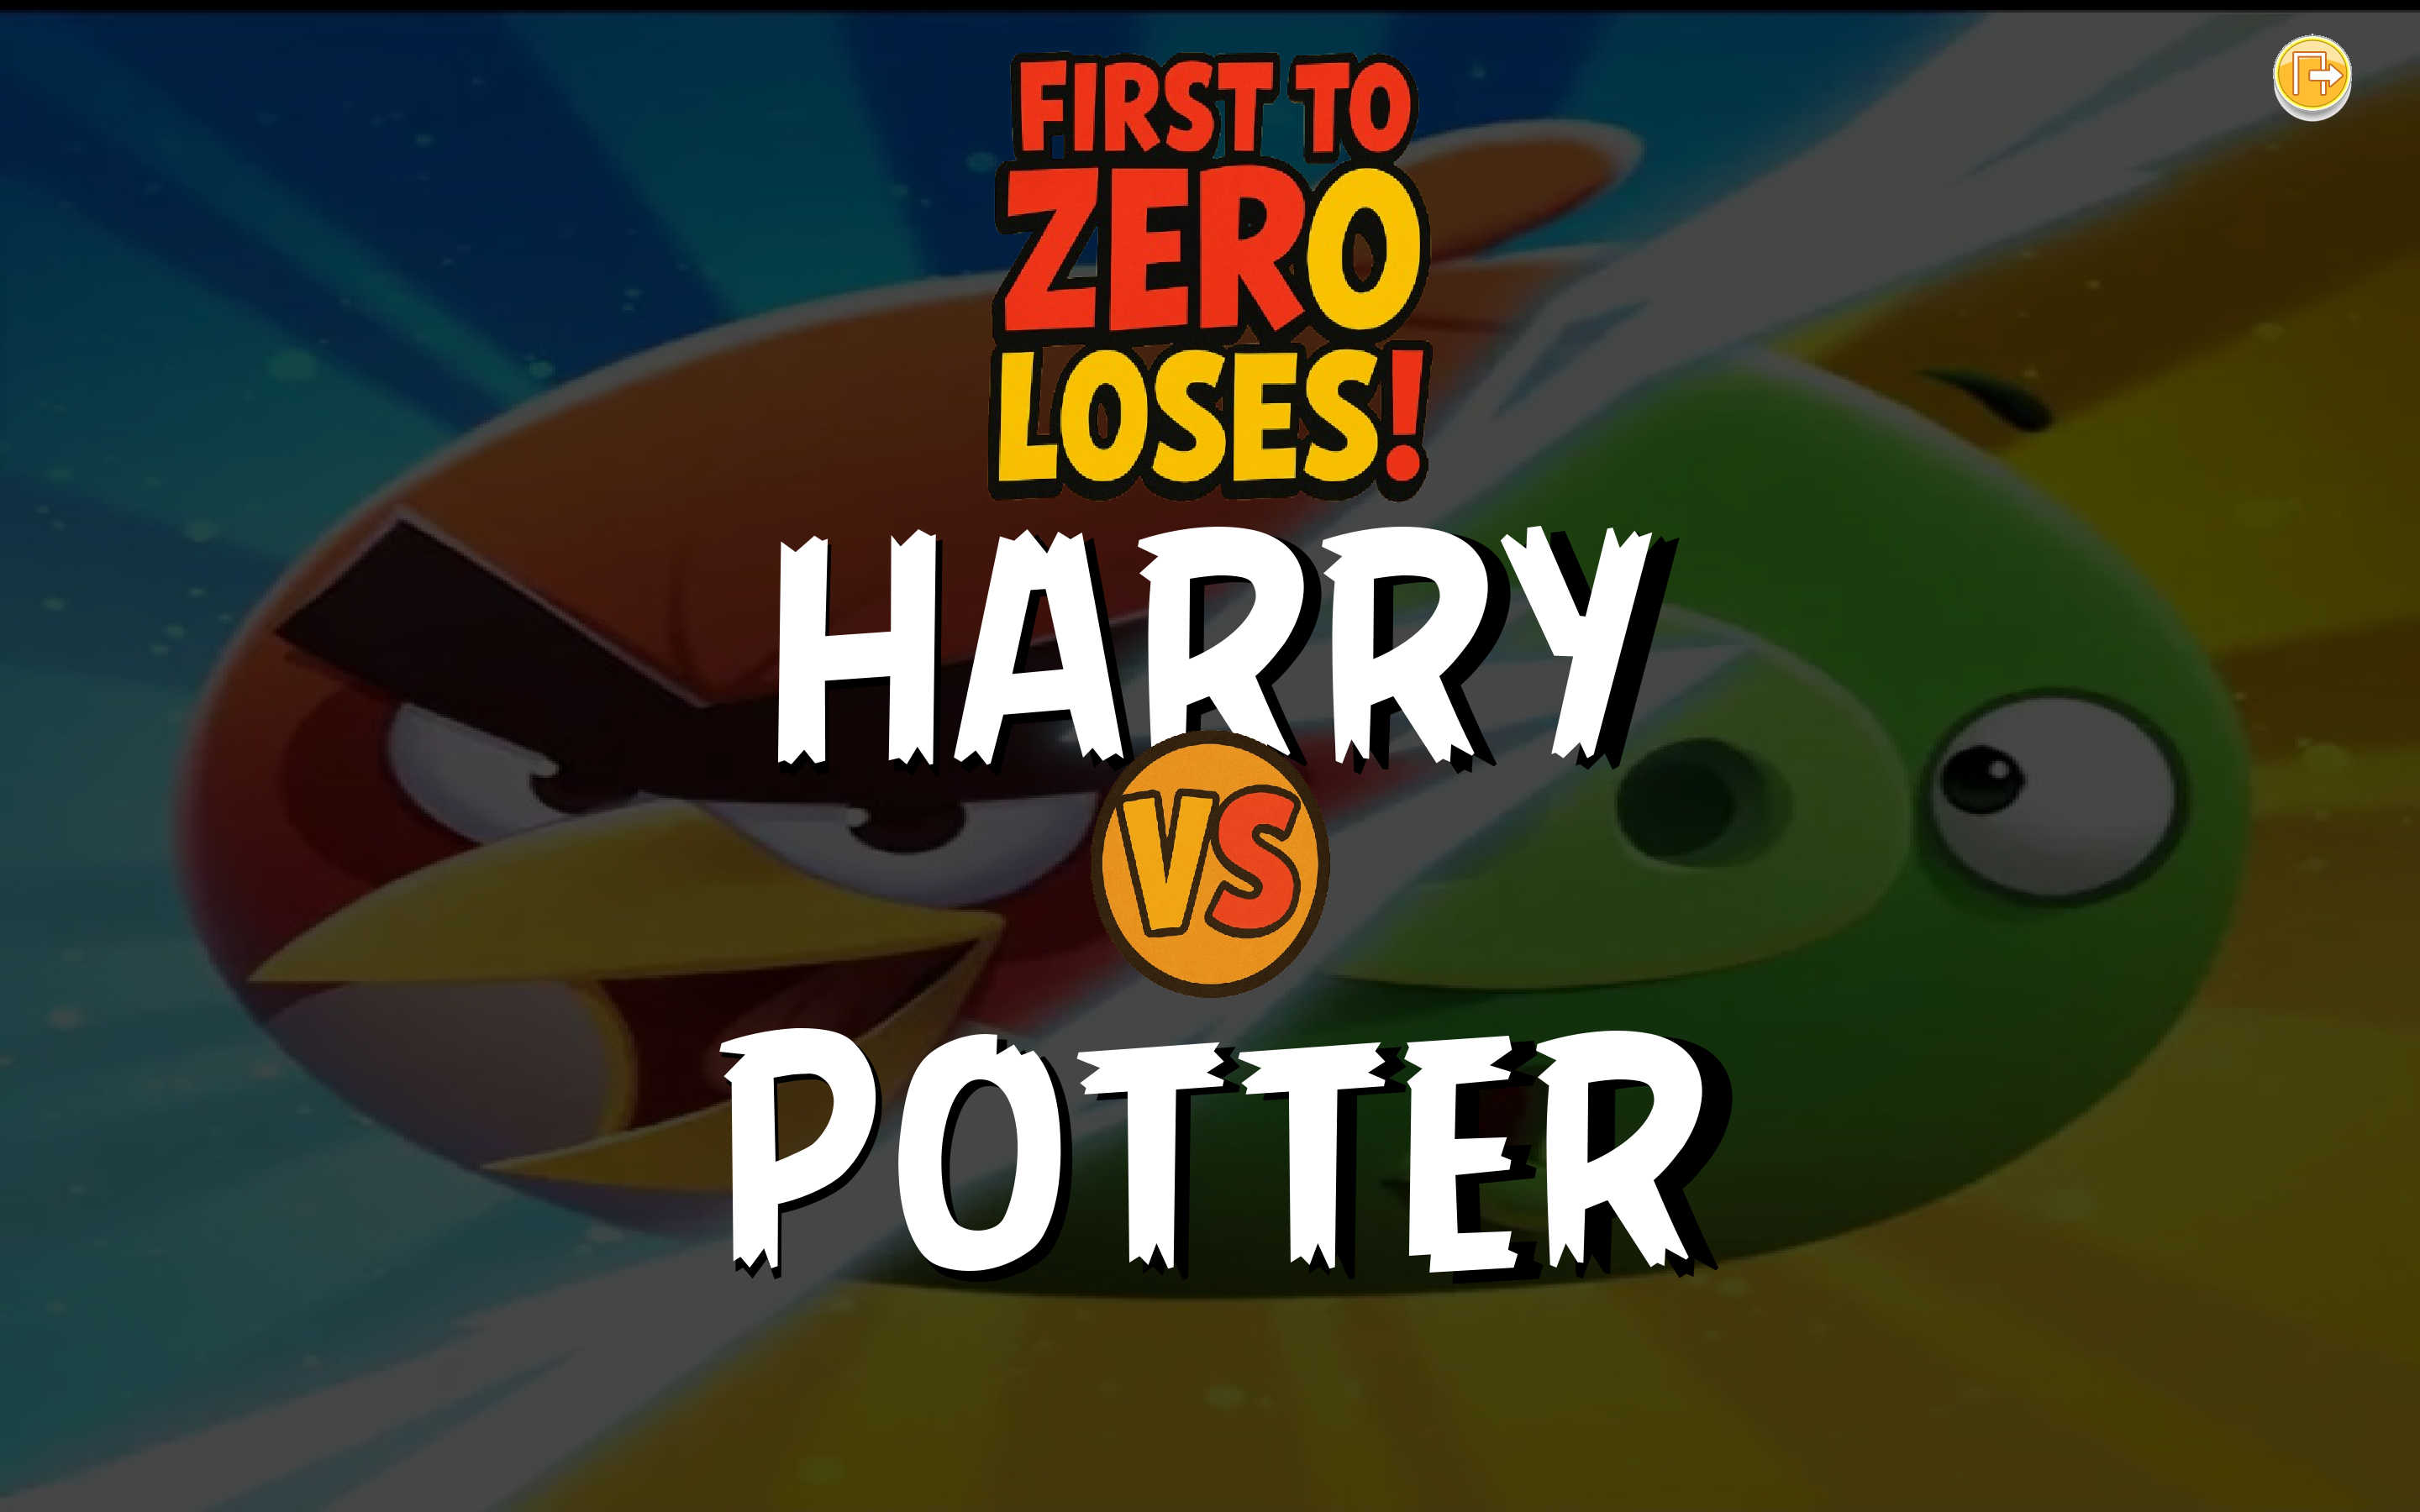
\includegraphics[width = 0.80\textwidth]{VS.png}
    \caption{VS}
    \label{fig:VS}
\end{figure}



\subsubsection{Game Starts}

\begin{itemize}
    \item \textbf{RETRY BUTTON}: Click to restart the match.
    \item \textbf{PAUSE BUTTON}: Click to pause the game.
    \item \textbf{WIND BUTTON}: Click at any point of time in the game to either 
    oppose the opponent projectile or benefit your own. You are only allowed to use it once per player.
\end{itemize}
\begin{figure}[h]
    \begin{minipage}[b]{0.4\linewidth}
        \centering
        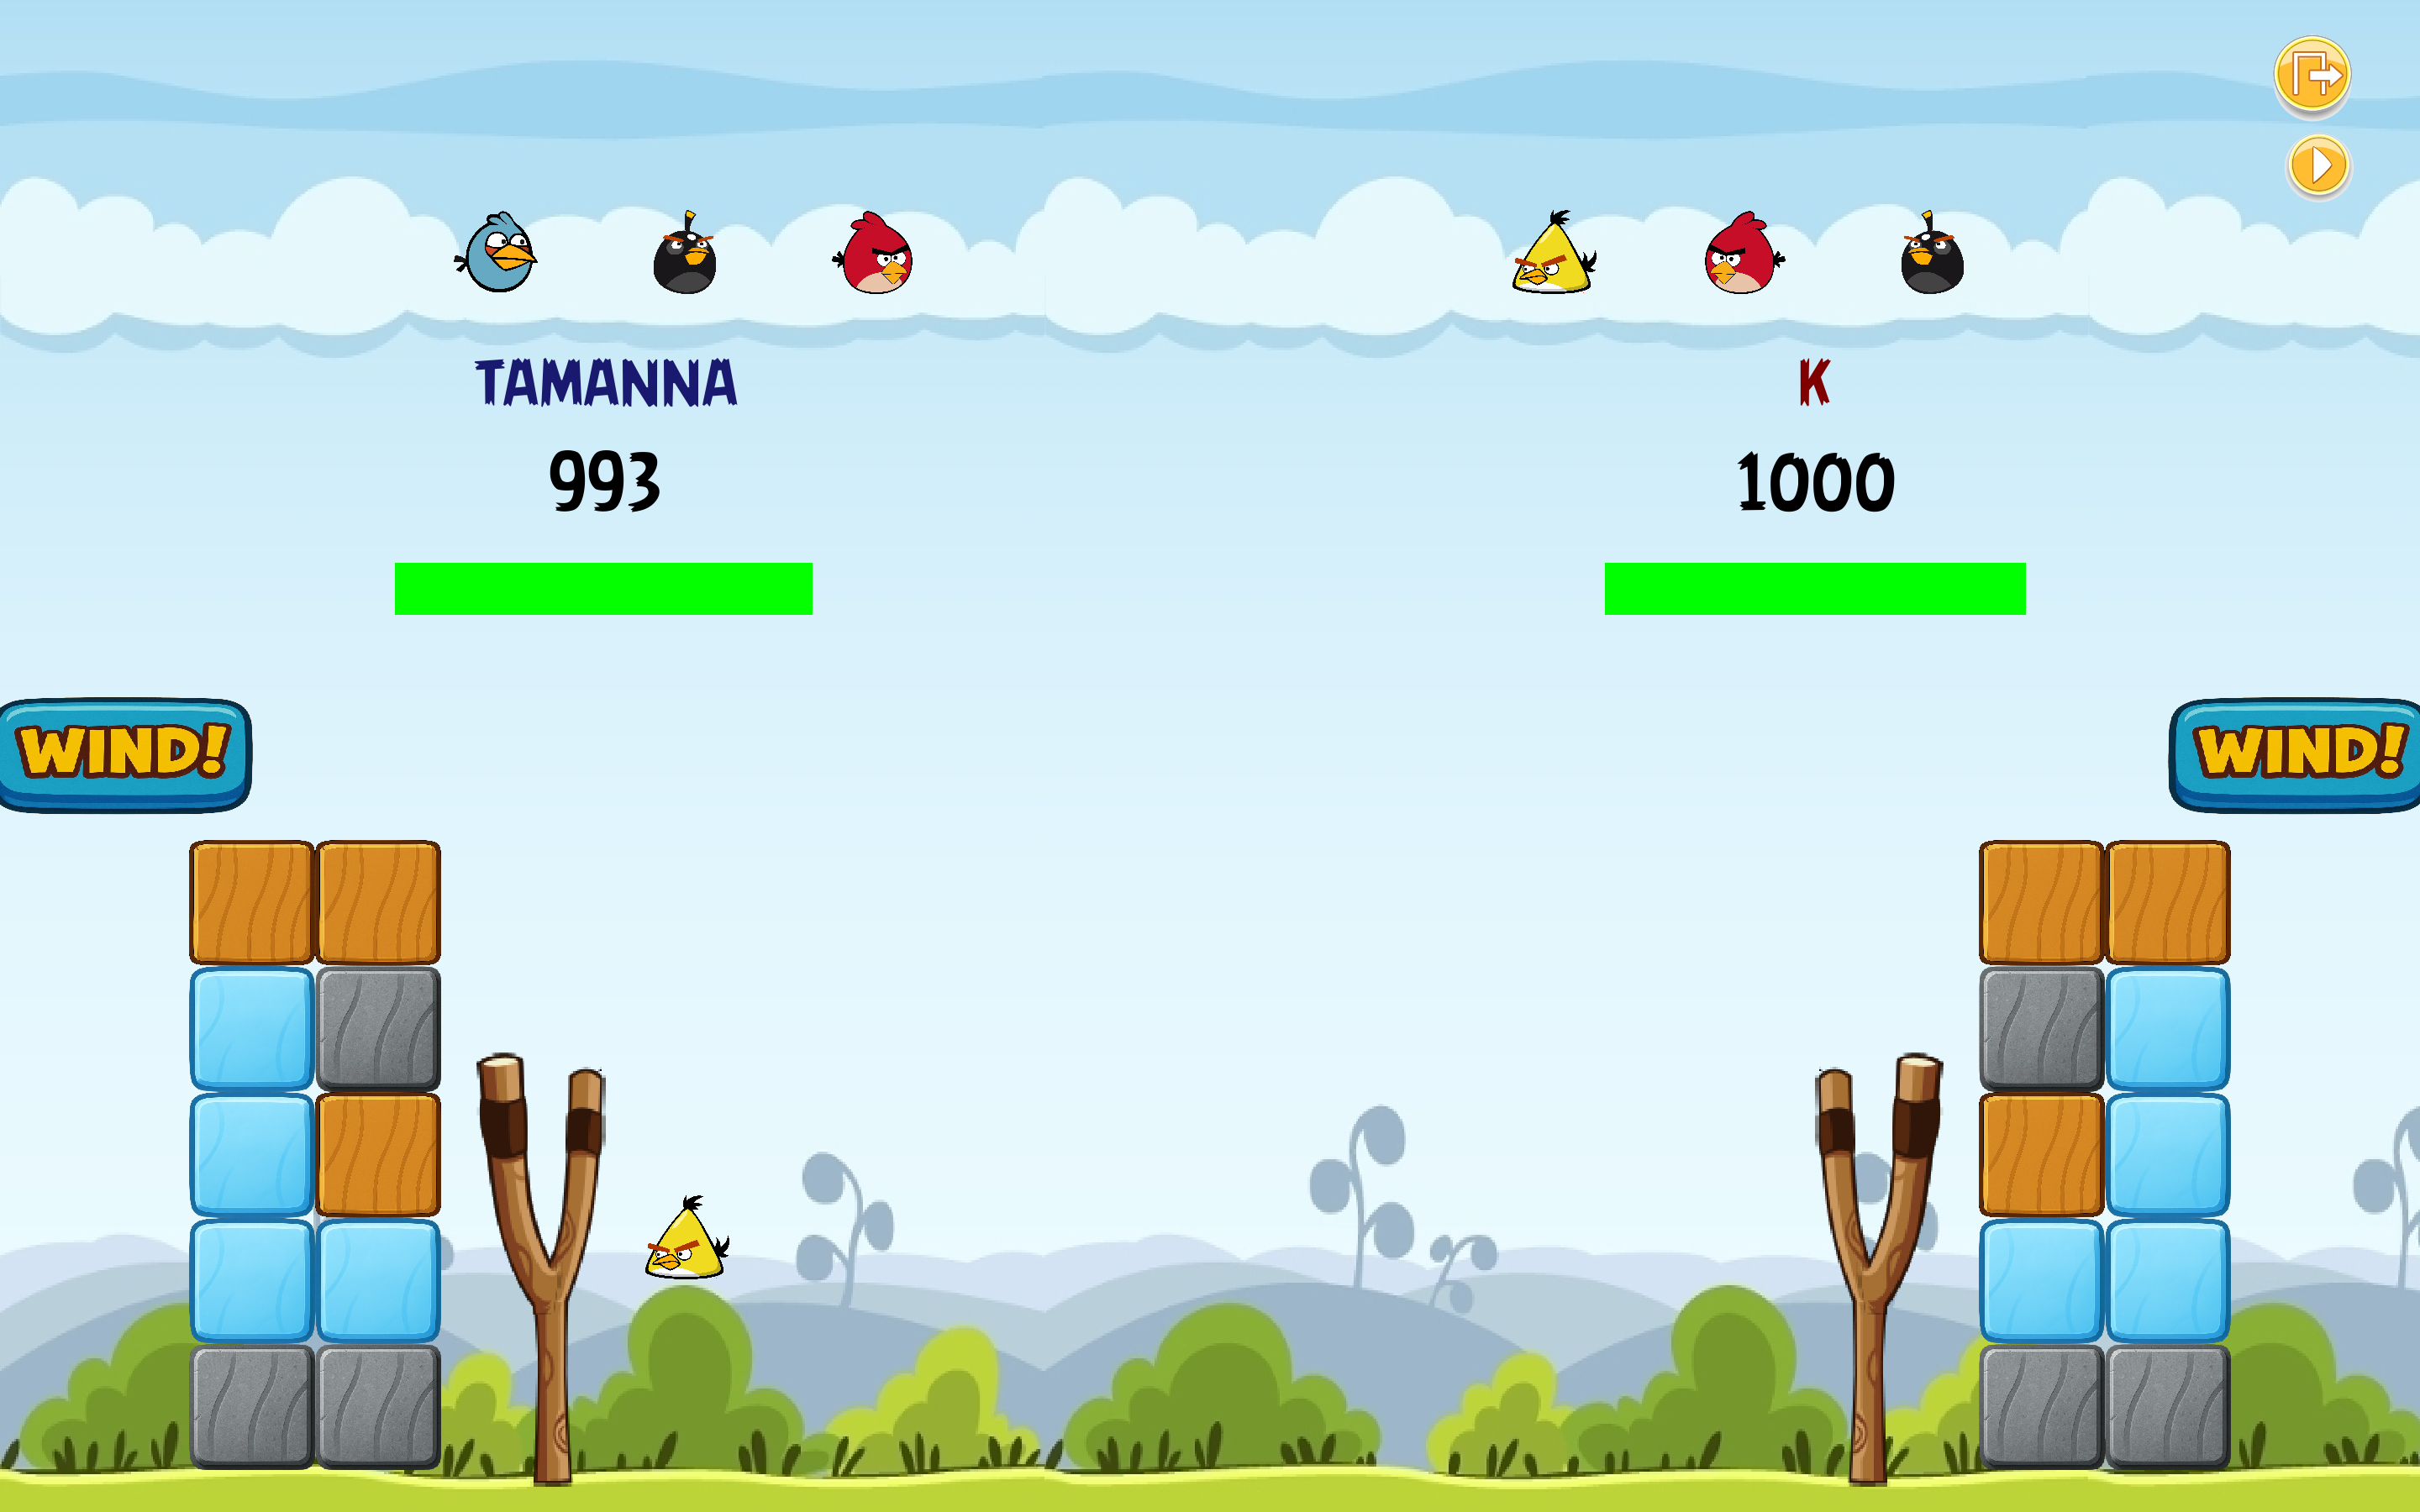
\includegraphics[width = 1\textwidth,left]{bird_projectile.png}
    \end{minipage}
    \hspace{0.25\textwidth}
    \begin{minipage}[b]{0.4\linewidth}
        \centering
        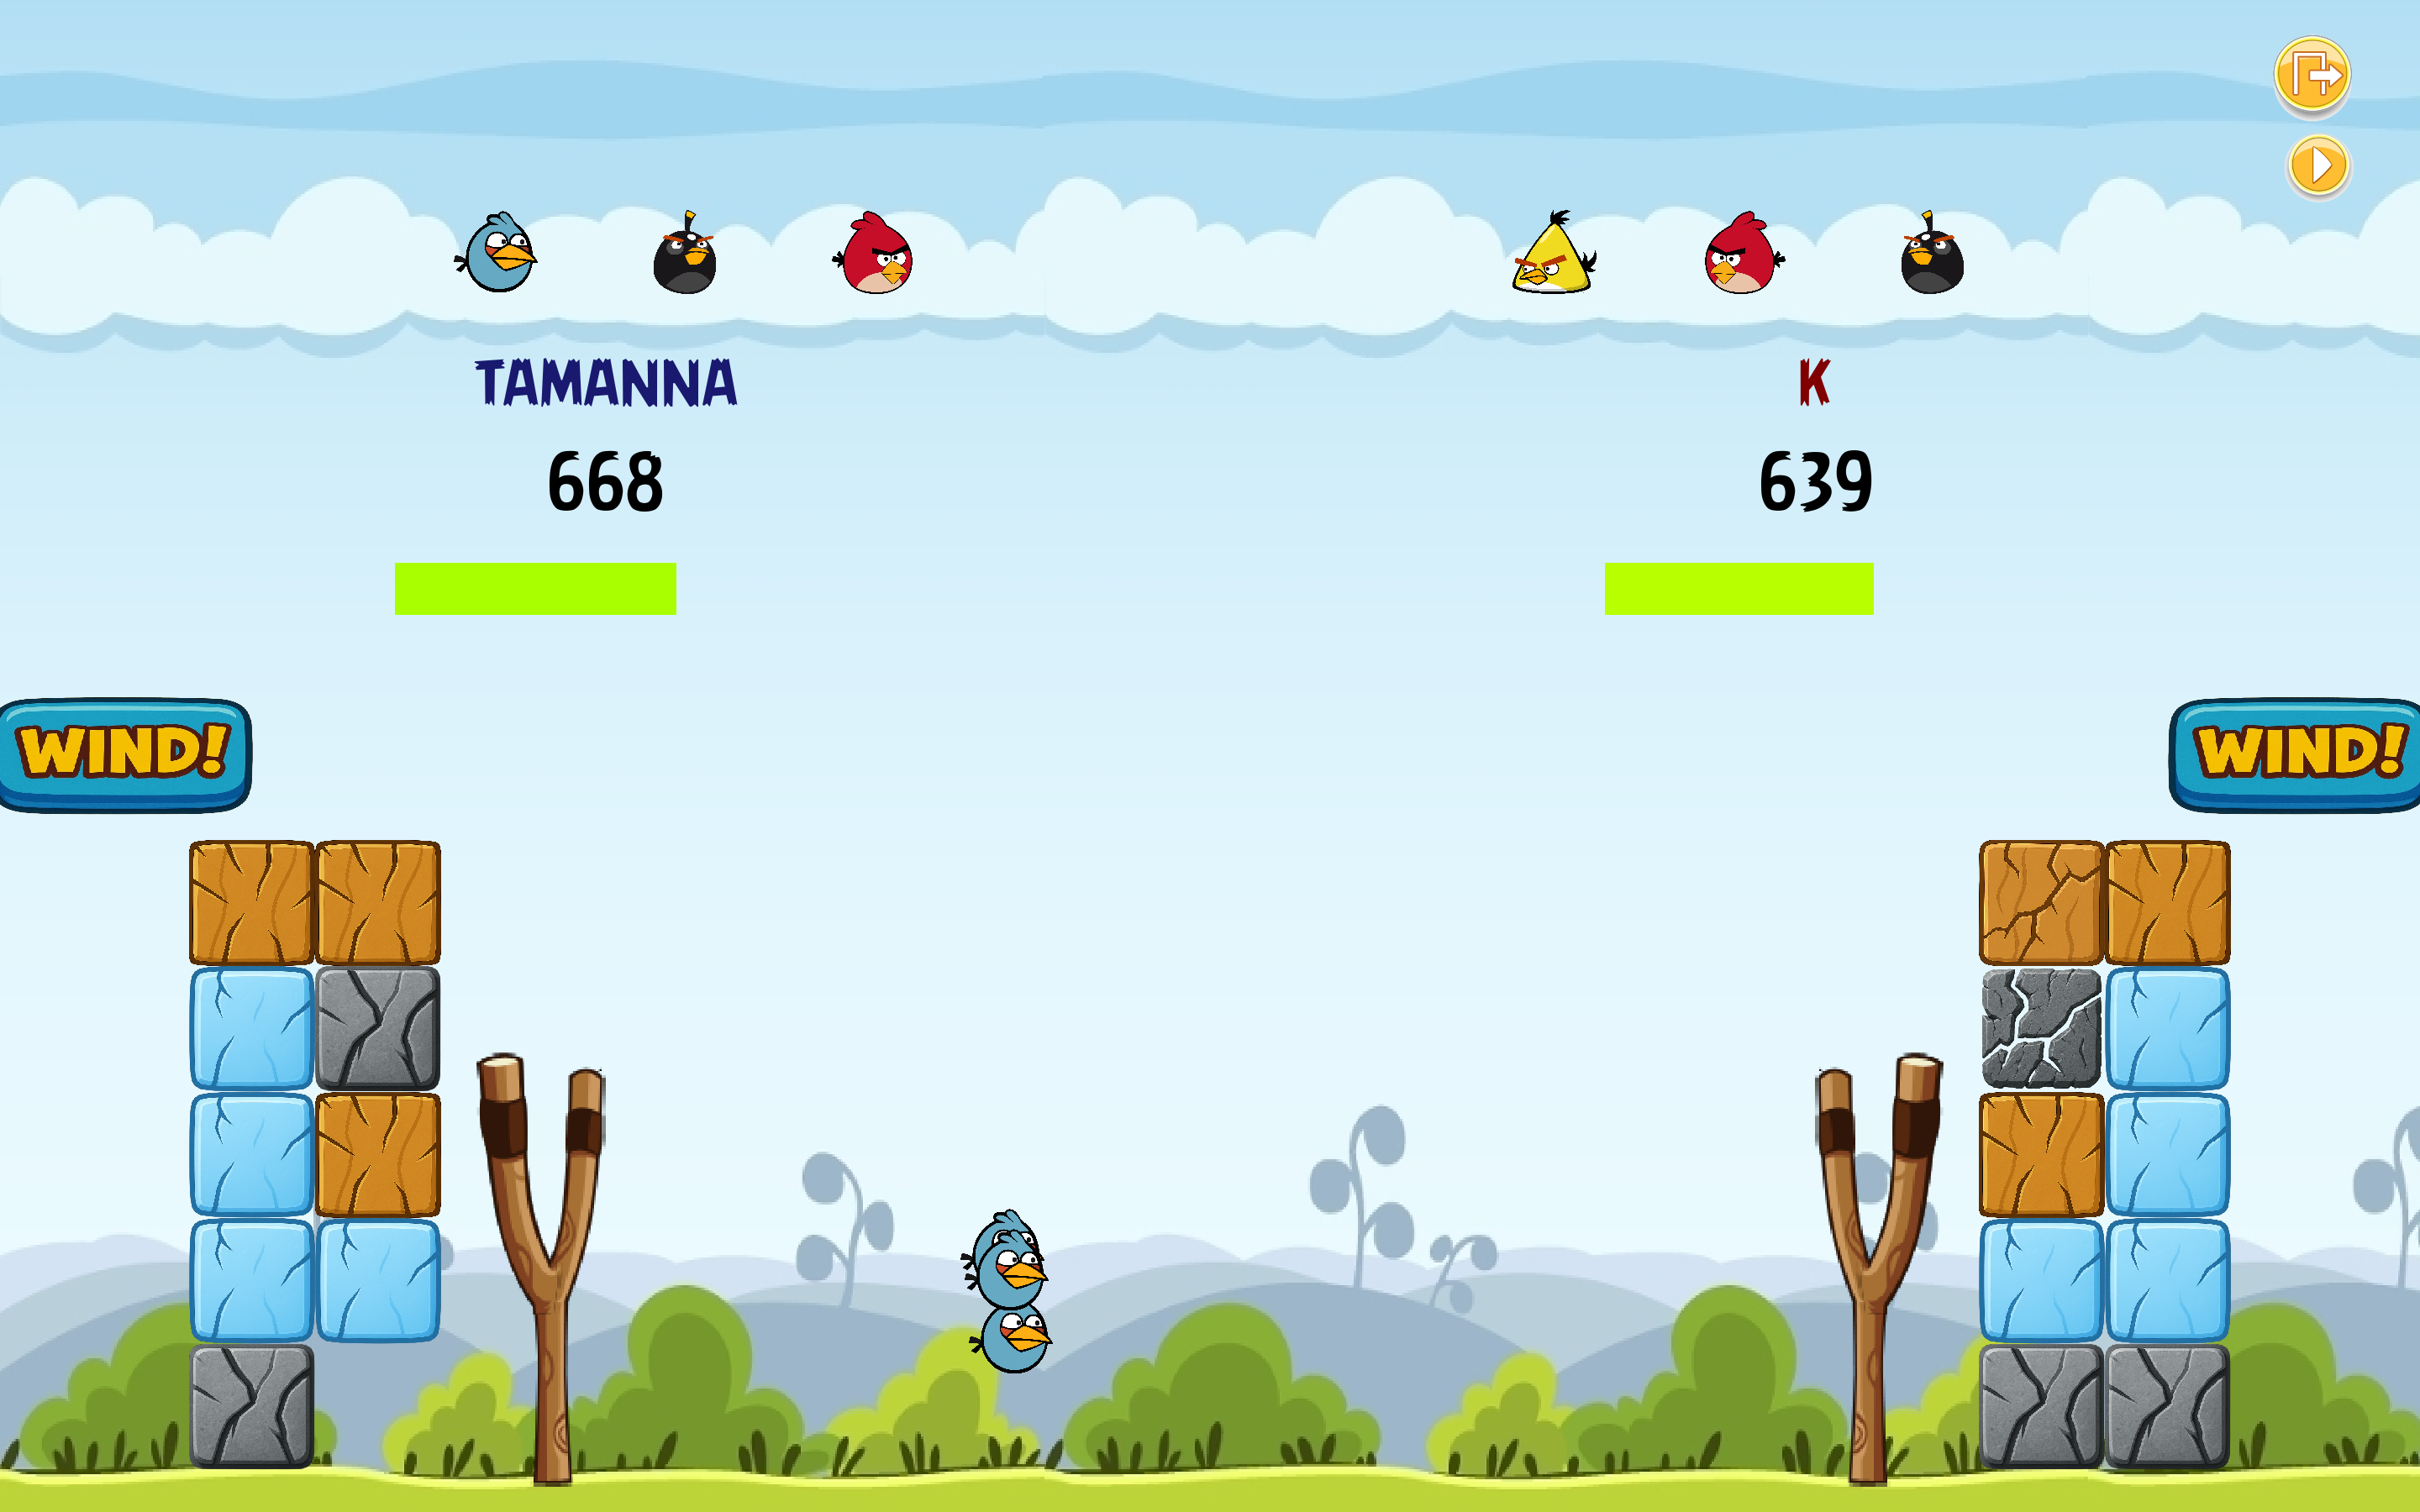
\includegraphics[width = 1\textwidth,left]{blue_triplify.png}
    \end{minipage}
    \caption{GAME PLAY}
    \label{fig:GAME_PLAY}
\end{figure}


\begin{figure}[h!]
    \centering
    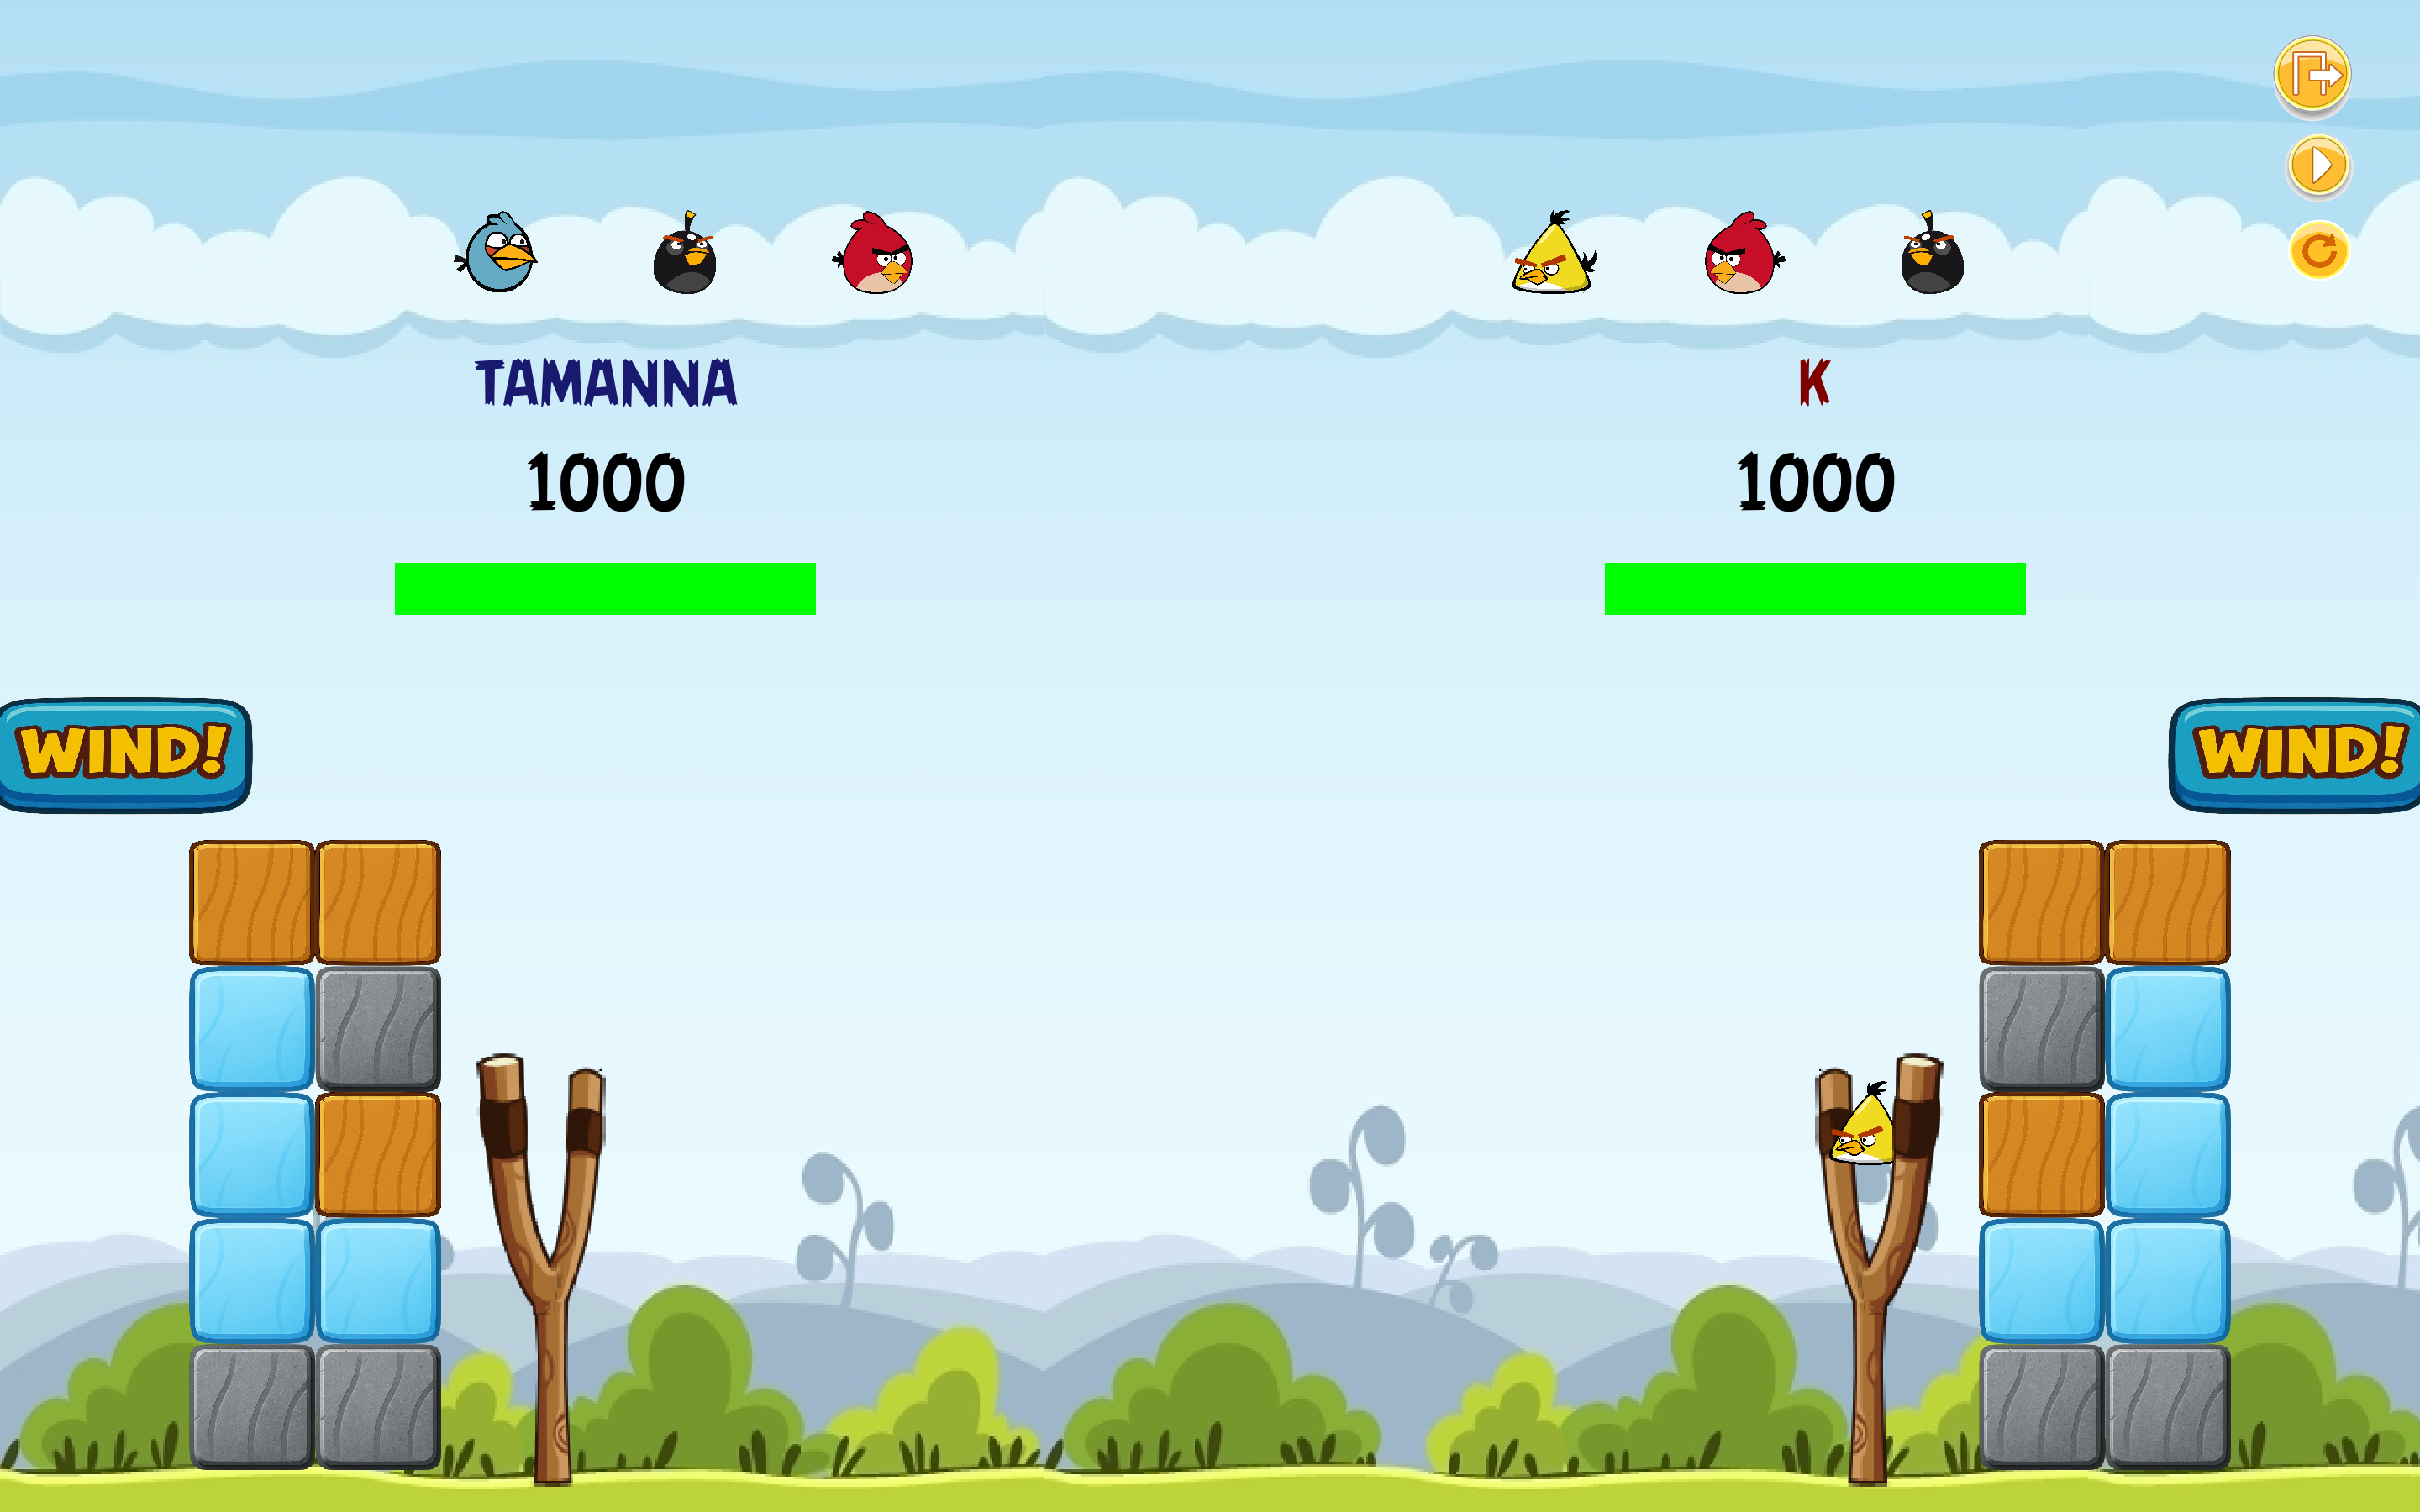
\includegraphics[width = 0.7\textwidth]{main_game.png}
    \caption{GAME INTERFACE}
    \label{fig:GAME_INTERFACE}
\end{figure}

\subsection{Playing the game}
The three birds that you choose keep circulating one by one. Drag and release the mouse to launch the bird.
A trajectory is shown for some distance between the sling and the block based on which you can aim at the blocks.

\subsection{Game Over}

First Player To 0 health loses.
\begin{figure}[h!]
    \centering
    
\includegraphics[width = \textwidth]{game_over.png}
    \caption{GAME OVER}
    \label{fig:GAME_OVER}
\end{figure}

A new game button pops up which restarts the program
\begin{figure}[h!]
    \centering
    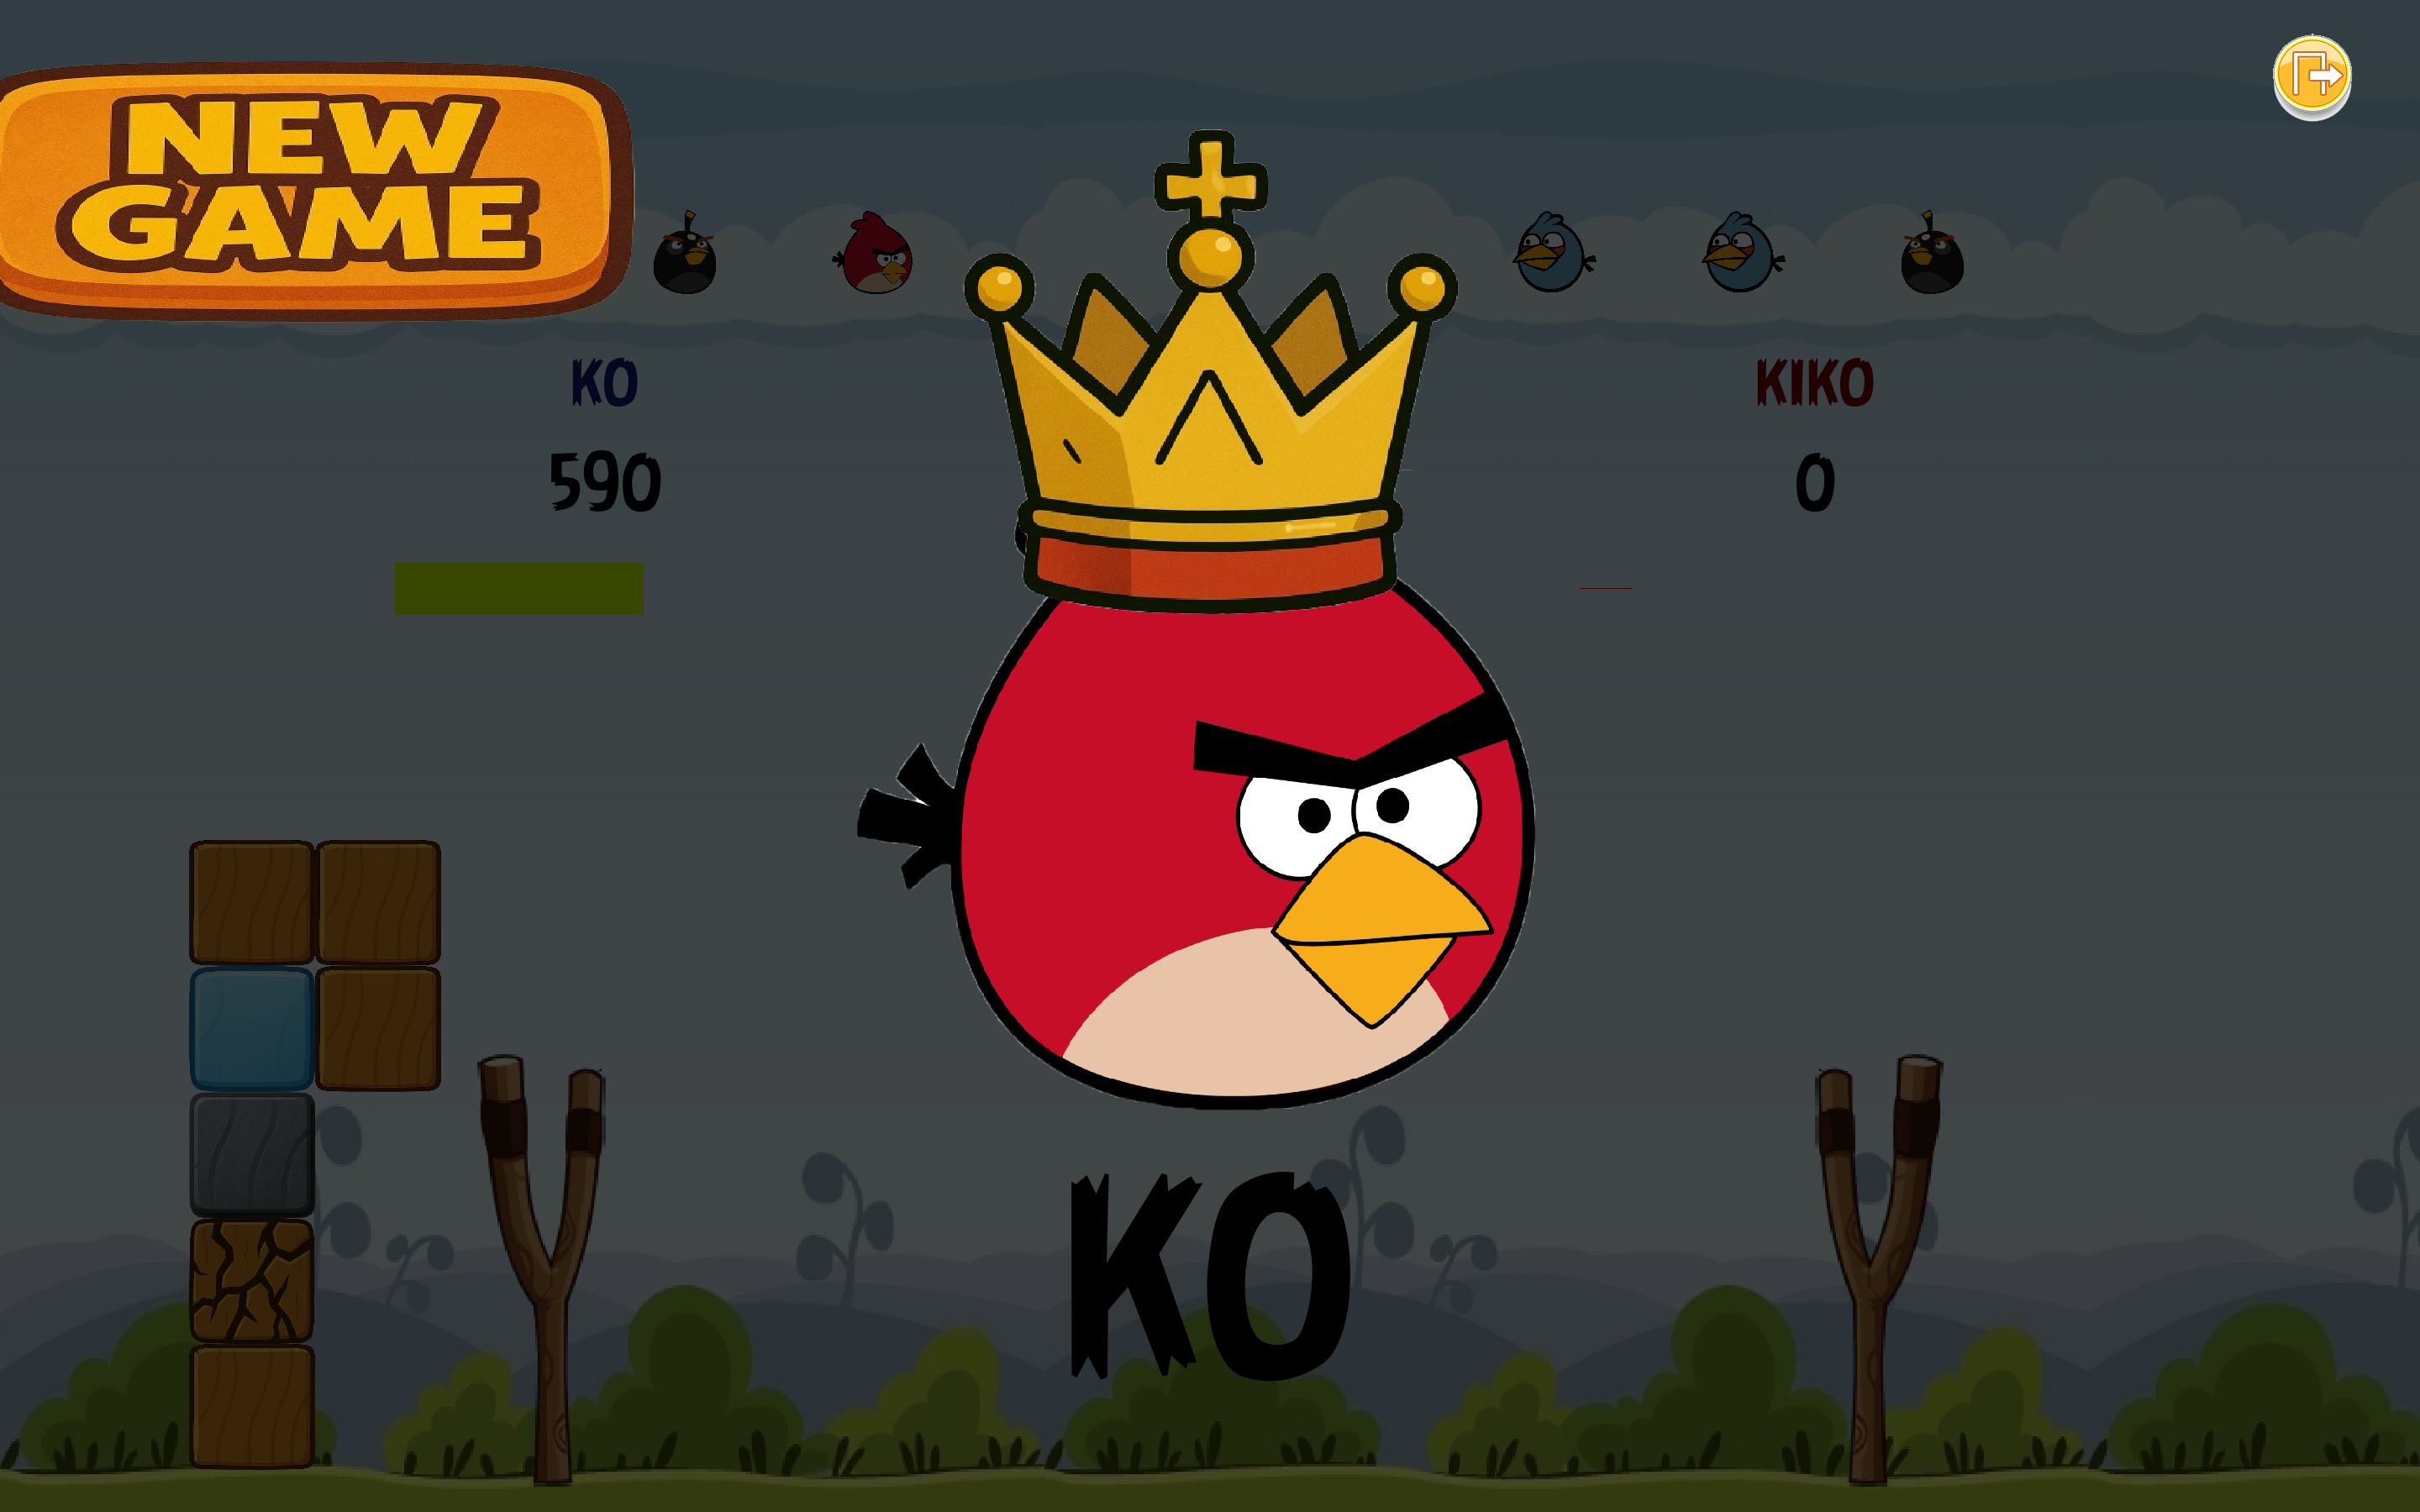
\includegraphics[width = \textwidth]{newgame.png}
    \caption{NEW GAME}
    \label{fig:NEW_GAME}
\end{figure}

\subsection{Various Implementations In The Code}

For Pygame functions I referred to the documentaion of 
pygame\cite{pygameDoc} and pygame-ce\cite{pygameCEDoc}
For sprite images I used reference image generation tools and open
source websites\cite{ImagesAndBGs}.
For inspiration, I went through some single-player Implementations
which helped me ideate and formulate my own game.\cite{ReferenceProjects}

\subsubsection{Customizations in the game}
A list of Customizations made in the game
\begin{itemize}
    \item Added special abilities for each of the birds
    \item Music and Sound
    \item Added WIND ability for the players
    \item Added various audio and image sources which make the game more dynamic.
    \item Customized Fonts
    \item Unique Bird Selection Menu.
    \item Added a Pause/Unpause Button 
    \item Added a retry button to restart a game from the beginning
    \item Added a new game button to make the game replayable.
    \item Added additional animations apart from the projectile.
\end{itemize}

\begin{thebibliography}{9}
    \bibitem{pygameCEDoc}
    Pyagme's Official Documentation
    \url{https://pyga.me/docs/}.

    \bibitem{pygameDoc}
    Pygame Official Documentation
    \url{https://www.pygame.org/docs/}.

    \bibitem{ReferenceProjects}
    Estevão Fonseca. *Angry Birds Clone in Python*. 
        
    \url{https://github.com/estevaofon/angry-birds-python}

    marblexu. *PythonAngryBirds*.

    \url{https://github.com/marblexu/PythonAngryBirds}.

    \bibitem{ImagesAndBGs}

    Tools (AI and non-AI) for images, backgrounds and audio.

    \url{chatgpt.com}

    \url{pinterest.com}

    \url{https://www.freeiconspng.com/images/angry-birds-png}

    \url{https://www.myinstants.com/en/index/in/}
\end{thebibliography}




\end{document}